\documentclass[pdftex,11pt,a4paper]{article}
\usepackage{blindtext}
\usepackage{graphicx}
\usepackage{subfiles}
\usepackage{amsmath}
\usepackage{amsthm}
\usepackage{tikz}
\usepackage{wrapfig}
\usepackage{lscape}
\usepackage{rotating}
\usepackage{epstopdf}
\usepackage[font=small,labelfont=bf]{caption}
\usepackage{hyperref}
\usepackage{color}
\usepackage{algorithm}% http://ctan.org/pkg/algorithms
\usepackage{algpseudocode}% http://ctan.org/pkg/algorithmicx
\hypersetup{
    colorlinks=true,
    linkcolor=blue,
    citecolor=blue
}
\usetikzlibrary{shapes.geometric, arrows}
\theoremstyle{definition}
\newtheorem{definition}{Definition}[section]
\newtheorem{theorem}{Theorem}[section]
\newtheorem{lemma}[theorem]{Lemma}
\theoremstyle{remark}
\newtheorem*{remark}{Remark}
\usepackage{amssymb}
\usepackage{amsfonts}
\usepackage{mathtools}
\usepackage{geometry}
 \geometry{
 a4paper,
 total={210mm,297mm},
 left=30mm,
 right=30mm,
 top=30mm,
 bottom=35mm,
 }
\newcommand{\defeq}{\vcentcolon=}
\newcommand{\eqdef}{=\vcentcolon}
\newcommand*{\V}[1]{\mathbf{#1}}%
\newcommand{\norm}[1]{\left\lVert#1\right\rVert}
\newcommand{\justif}[2]{&{#1}&\text{#2}}
\newcommand{\qedwhite}{\hfill \ensuremath{\Box}}
\newcommand\given[1][]{\:#1\vert\:}
\newcommand{\me}{\mathrm{e}}
\DeclarePairedDelimiterX{\infdivx}[2]{(}{)}{%
  #1\;\delimsize\|\;#2%
}
\DeclarePairedDelimiter\abs{\lvert}{\rvert}%
\newcommand{\Conv}{\mathop{\scalebox{1.5}{\raisebox{-0.2ex}{$\ast$}}}}%
\newcommand{\infdiv}{\infdivx}
\renewcommand{\qed}{\hfill\blacksquare}
\hyphenation{op-tical net-works semi-conduc-tor tech-no-lo-gy}


\begin{document}
\title{Learning relational structures from birdsong}
\author{Authors,~a}

\maketitle


\begin{abstract}
We infer phylo-acoustic trees (relational structures built from acoustic similarity) for over 80 bird species in the British Isles. We characterise each bird species as a statistical model (either a probability distribution function or a Variational Bayes Hidden Markov Model) trained on birdsong excerpts and then use their pairwise similarity to build a phylo-acoustic tree by running Agglomerative Hierarchical Clustering. In order to achieve this, we define similarity metrics for HMMs, hence implicitly defining a \emph{length-invariant} method to compare birdsong across different species. Additionally, we show that there is a clear community structure in the resulting phylo-acoustic trees.
\end{abstract}


\section{Introduction}
\label{section_introduction}
The explosion of data in recent years has allowed scientists to gain insight in a diversity of domains. Furthermore, the widespread use of computational methods has in turn provided means of rapidly extracting conclusions from data. For example, environmental scientists have been allowed to contribute to quantify environments by means of \emph{unsupervised learning} techniques, which aim to provide insight on the hidden structures of data. Quantifying environments is crucial in order to analyse phenomena in a formal manner.
\par In this work, we tackle the problem of describing a hierarchical structure of bird species only by means of their birdsong. This mathematical representation relies only on the validity of a formal analysis framework, and hence unveils relations that go beyond empirical conclusions. This phylo-acoustic tree may further our understanding of relations among bird species in a large geographical area, and bird evolution over a large span of time. 
\par Birdsong is a rich means of communication that encapsulates behavioural patterns (such as territory defence and mate attraction or competition \cite{Berwick2013, Naguib2014}) in a regular and hierarchical fashion \cite{Snowdon2013}, as shown in figure \ref{fig_birdsong_structure}. Crucially, birdsong is learnt by repetition \cite{Berwick2013}, which implies that forced migration may push flocks to learn songs that do not necessarily come from their parents. Hence, building phylo-acoustic trees may further our understanding of how different species are related (even across different genera).
\begin{figure}[t]
\centering
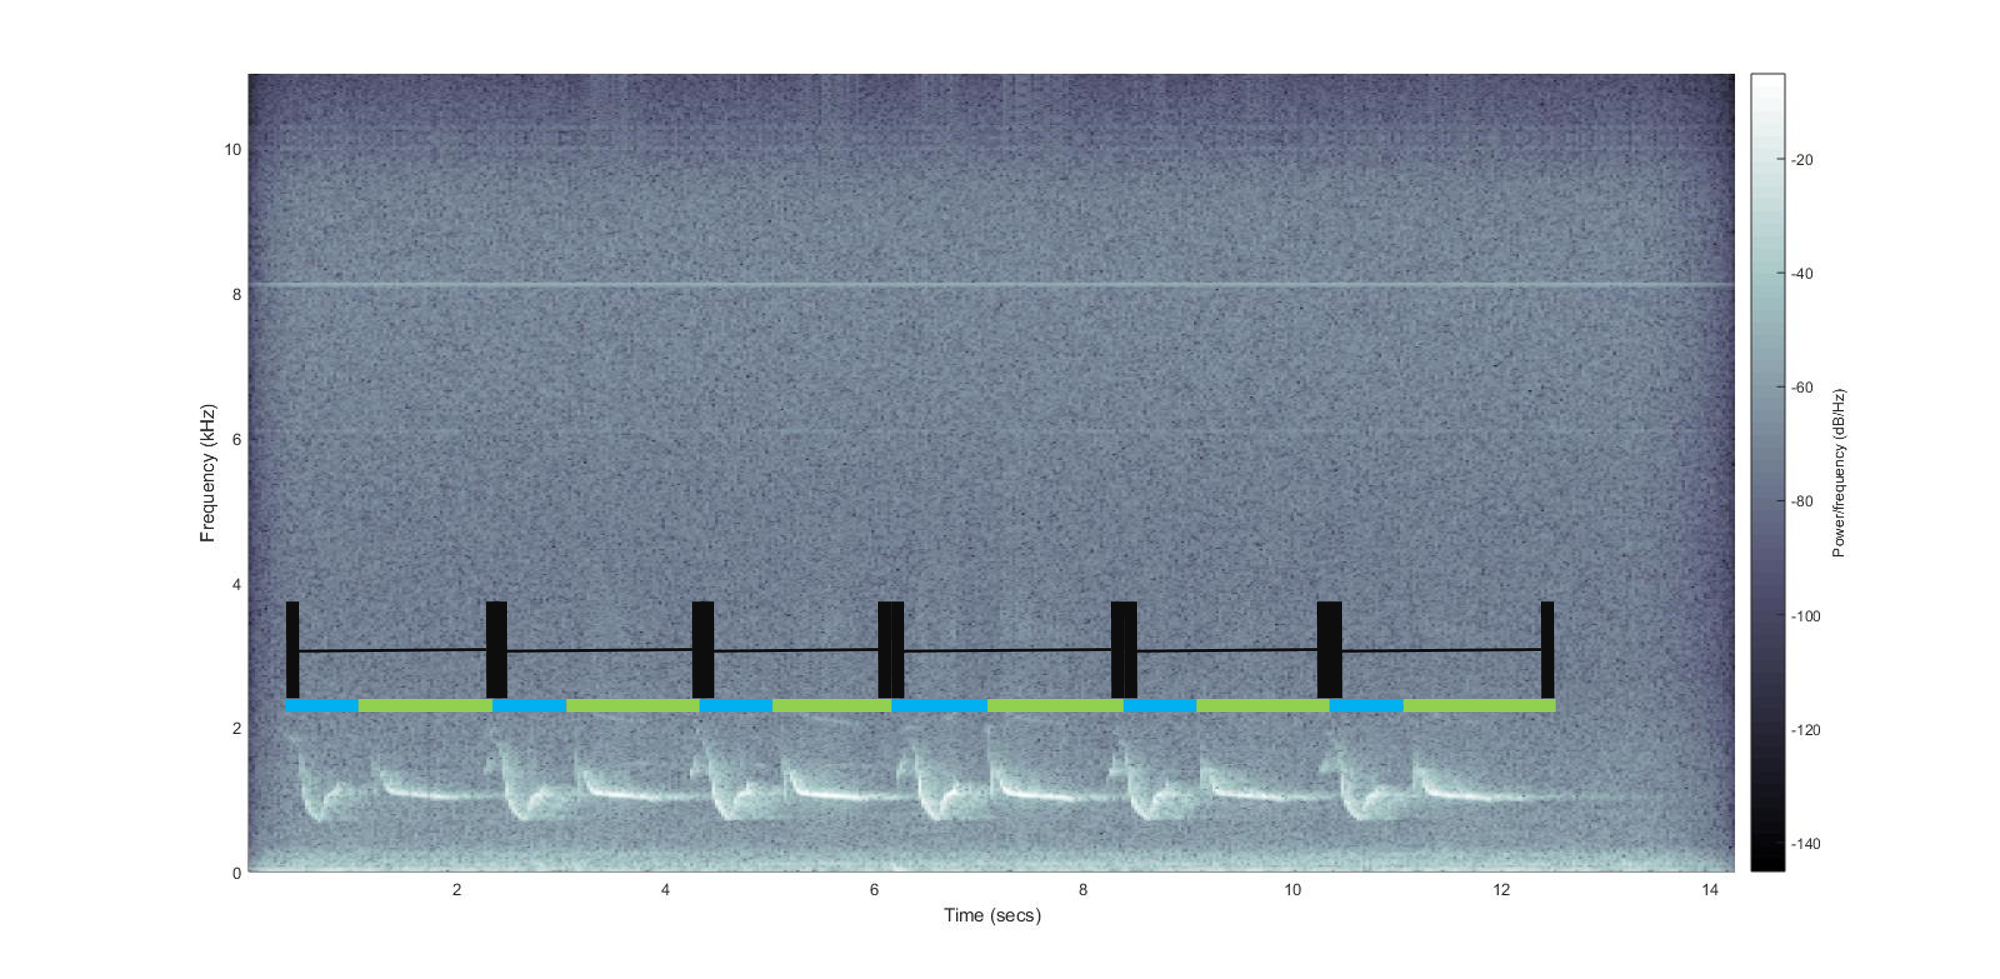
\includegraphics[width=\textwidth]{images/birdsong_structure}
\caption{Spectrogram from a birdsong recording of the species \emph{Periparus ater}. Remark the regular structure of birdsong: syllables (thick boxes) are composed of motifs (thin boxes).}
\label{fig_birdsong_structure}
\end{figure}
\par Importantly, several academics in Zoology have pointed out the similarities between human speech and birdsong, e.g. we can think of both humans vowels and birdsong as ``complex, patterned vocalisations" \cite{Berwick2013,Naguib2014}. This remark enables us to analyse birdsong by means of some of the techniques from the field of Automatic Speech Recognition (ASR), which will be introduced in section \ref{section_model}. 
\par The rest of this article is organised as follows: in section \ref{section_model}, we introduce the mathematical framework used to build phylo-acoustic trees; then, in section \ref{section_results}, we present our experiments and results; and in section \ref{section_conclusion} we present our conclusions and future work.

\section{Model architecture}
\label{section_model}
In this section, we describe a procedure to build phylo-acoustic trees given a dataset $\mathcal{D}$ with audio recordings of birdsong of different bird species from a set $X$. We are interested in finding a relation $R$ over pairs of elements in $X$, along with a scalar $s_{i, j} \in \mathbb{R}$ called the \emph{similarity} between species $s_i, s_j \in S$, i.e. $R \subseteq S \times S \times \mathbb{R}$. This relation can then be expressed as a symmetric matrix $A = (d_{i,j})$ and be used as input to build a phylo-acoustic tree by means of Agglomerative Hierarchical Clustering (AHC). 
\par Due to the continuous nature of birdsong, recordings in $\mathcal{D}$ are rarely of the same length, and hence we would like to build a similarity matrix that is \emph{length-invariant}. We achieve this by characterising each bird species $s_k \in S$ as a statistical model, and then by defining a similarity metric between pairs of statistical models. In the rest of this section, we aim to describe how to train such models, and then explain how they can be used in conjunction with AHC to build phylo-acoustic trees.
\par In our work, we associate each bird species to a statistical model on the frequency components of their birdsong. In order to extract frequency features from birdsong, we use the Linear Predictive Coding (LPC) framework to compute the \emph{formant trajectories} of each birdsong recording. The LPC framework is based on the source-filter model of speech, which models acoustic signals shaped by the vocal tract, such as vowel sounds shaped by the larynx in the case of humans, and as birdsong, which is shaped by the syrinx.

\subsection{Feature extraction}
\par \textcolor{red}{\textbf{At least mention some of the techniques you didn't use.}} 
The signal processing literature provides a broad range of techniques that can be used to extract features from acoustic signals. 
Formant trajectory extraction is based on the Linear Prediction of Speech framework \cite{Snell1993}. Consider a short excerpt of birdsong (20-40ms) $\V{s}$. Then, it is described by the LTI system with system function:
\begin{align*}
H(z) = \frac{1}{A(z)} = \frac{1}{1-\sum_{i=1}^pa_iz^{-i}}
\end{align*}
where 
\begin{align*}
\sum_{i=1}^pa_iz^{-i} = \V{\hat{s}}
\end{align*}
is the $p$-th order autoregressive approximation $\V{\hat{s}} = \V{s} - \V{\hat{e}}$. Remark that this LTI system is fully characterised by the coefficients $a_i$. We now define the formant frequencies of the excerpt $\V{s}$ as the poles of the system function $H(z)$; intuitively, these can be thought of as the resonances of the vocal tract of each bird when generating birdsong. Now, given a pair of complex roots $re^{\pm\theta}$, the formant frequency associated to it is given by:
\begin{align*}
F = \frac{f_s}{2\pi}\theta \text{Hz}
\end{align*}
where $f_s$ is the sampling frequency of the signal. Furthermore, the 3-dB bandwidth associated to it is:
\begin{align*}
B = -\frac{f_s}{2\pi}\log{r} \text{Hz}
\end{align*}
\par Another way of interpreting formants is as the peaks of the spectral envelope of the signal. This gives an intuition to the 3-dB bandwidth, which is simply the width of envelope exactly 3 dB below the peak. Smaller bandwidths hint at clearer, more characteristic formants. By framing the original birdsong recording into small excerpts and repeating the procedure above, we obtain a trajectory of formants extracted uniformly over small intervals of time. Figure \ref{fig_specformants} shows the trajectory of the first non-zero formant for a birdsong recording.

\begin{figure}[t]
\centering
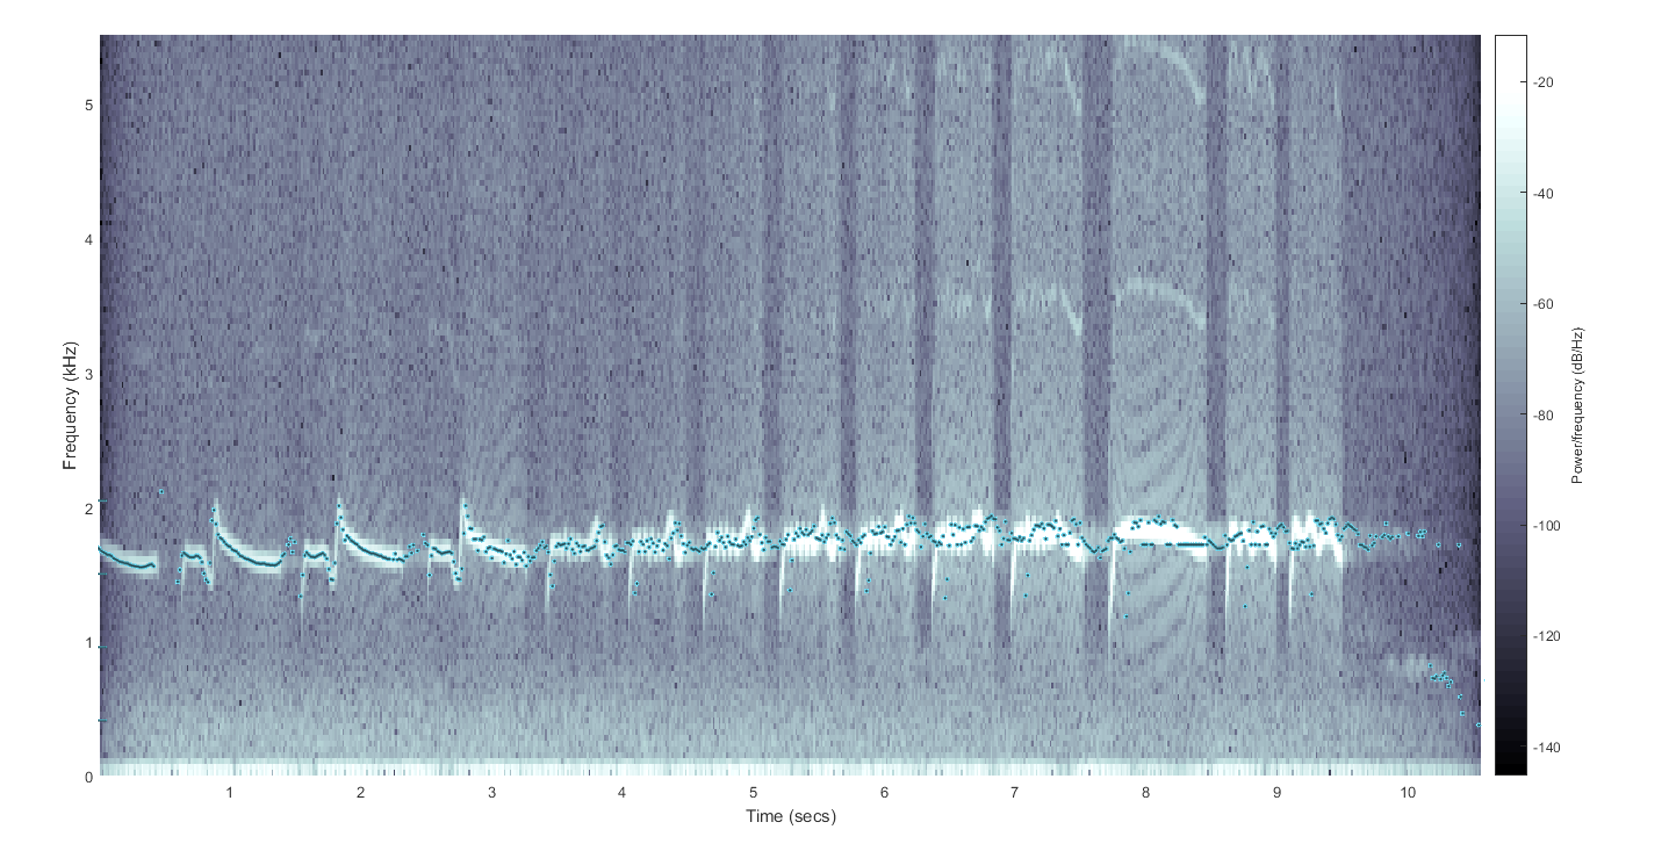
\includegraphics[width=\textwidth]{images/formants}
\caption{Depiction of the first non-zero formant trajectories (blue) on top of a birdsong recording spectrogram of the species \emph{Periparus after}. Remark how the trajectory corresponds to the white bands (sections with a larger amount of energy) of the spectrogram.}
\label{fig_specformants}
\end{figure}

\subsection{Training statistical models}
Once each birdsong recording has been transformed into a formant trajectory, we can train models that characterise each bird species as a function. In particular, we describe methods to estimate probability distributions and to train Variational Bayes Hidden Markov Models (VB HMM).

\subsubsection{Kernel Density Estimation}
\par KDE consists in approximating the probability density function of a set of points as a linear combination of basis functions (non-negative kernels). We place an instance of this basis function around each point in the set, add them up and normalise. For the univariate case, the pdf $p_K(x)$ obtained from KDE using kernel $K$ over a set of points $X$ is given by:
\begin{align*}
p_K(x) = \frac{1}{Nh}\sum_{i=1}^NK\left(\left|\frac{x - x_i}{h}\right|\right)
\end{align*}
where $h$ is called the bandwidth. Crucially, using a smooth kernel provides a smooth pdf as a result, where the degree of smoothness is controlled by the parameter $h$, and its value will make the resulting probability function be oversmoothed, undersmoothed or optimally smoothed.
\par One of the most common smooth kernels in the literature is the univariate Gaussian kernel \cite{hastie2008}, given by:
\begin{align*}
K_G\left(\frac{x}{h}\right) = \frac{1}{\sqrt{2\pi}}\exp{\left(-\frac{x^2}{2h^2}\right)}
\end{align*}
whose optimal bandwidth in the least-squares error sense is given by $h = \hat{\sigma}n^{-1/5}$, where $\hat{\sigma}$ is the standard deviation of the sample $X$.
\par Note that, despite its simplicity, KDE is a poorly scalable strategy: on one hand, the bandwidth $h$ becomes harder to choose as the dimensionality of data increases \cite{Hansen2009}; additionally, the space required to store the output pdf increases exponentially with each added dimension.

\subsubsection{Gaussian Mixture Models}

\label{subsection_gmm}
The scalability challenge imposed by KDE motivates the look for a more compact representation of data. Note that formant trajectories for different birdsong syllables from the same species have been shown to exist in different frequency ranges. This suggests the existence of subpopulations in our data $\mathcal{X}$. In this case, we can use a smaller number of basis functions. This can be achieved by means of a Gaussian Mixture Model (GMM), which is a convex combination of Gaussians (called \emph{mixtures}). In other words, the pdf fitted to the data takes the form:
\begin{equation} \label{eq:mixmod}
p(\V{x} \given \theta ) = \sum_{i=1}^K\pi_i \mathcal{N}(\V{\mu}_i, \Sigma_i) 
\end{equation}
with $\sum_i=1^K\pi_i, 0 \leq \pi_i\leq 1$. Nevertheless, even if GMMs are more scalable than KDE, neither method allows for the existence of time ordering of data. That is, both models treat the formant trajectories as sets, rather than sequential structures. This motivates the need for an even more abstract structure that takes into consideration the sequential structure of formant trajectories.

\subsubsection{Variational Bayes Hidden Markov Models}
\label{sub_hmms}
Although Gaussian Mixture Models overcome the scalability issues of KDE, both techniques still suffer from losing the sequential structure of formant trajectories. Hidden Markov Models overcome these challenges by combining an \emph{emission model} with parameters $\phi$, a \emph{transition model}, which is a Markov chain with transition matrix $B$, and an initial state categorical distribution $\pi$, which altogether describe a sequence $\V{x}$: the emission model explains the observations in the sequence, whereas the transition model and the initial state distribution explain its time ordering.
\par In this scenario, we aim to infer the probability that the model generated such observations $\V{x}$ and that the underlying Markov Process generated the sequence of states $\V{s}$. This is given by the joint probability $p(\V{x}, \V{s})$:
\begin{equation}\label{eq:hmm}
p(\V{x}, \V{s}) = p(\V{s})p(\V{x} \given \V{s}) = p(s_1)\prod_{t=1}^{T-1}p(s_{t+1}\given s_t)\prod_{t=1}^Tp(\V{x}_t \given s_t)
\end{equation} 
\par An HMM is fully characterised (up to a permutation of states) by these three parameters $\theta = (\phi, B, \pi)$. Furthermore, the observations analysed by an HMM can be continuous or discrete \cite{Jurafsky2009}. Note that formants $\V{f}_i$ belong to a continuous space, hence we will focus on describing continuous HMMs henceforth.
\par Let the emission model of an HMM be a GMM. Notice that the transition model explains the data's sequential structure without losing any of the GMM's advantages described in section \ref{subsection_gmm}. Thus we have overcome the main challenge described for GMMs. However, we still have two matters to address: on one hand, we have yet to describe a learning procedure for continuous HMMs; on the other hand, we also have to touch on model selection, i.e. finding a method to choose how many states an HMM should have. Importantly, note that for every HMM with $K$ states, there exist $K!$ equivalent HMMs that can be generated by permuting the identities of the HMM's states. This problem is called \emph{identifiability} \cite{Bishop2006}, and will play an important role when we define a metric between HMMs. 
\par We first address HMM training. We aim to make inferences about the parameters $\theta$ given data $\mathcal{X}$. A \emph{frequentist} approach to this is Maximum Likelihood Estimation (MLE). However, MLE has several disadvantages \cite{Murphy2012}. Firstly, there is no measure of uncertainty regarding the point estimate $\hat{\theta}$, and thus we are not able to know how trustworthy the estimate is. Secondly, the mode of a distribution is often untypical of the distribution \cite{Murphy2012} because it does not take into account the volume distribution of the probability distribution. Finally, MLE estimates are prone to overfit data. To illustrate this scenario, consider a fair coin that is tossed two times, and it lands heads on both occasions. An MLE estimate for this Bernoulli distribution would set $\hat{\theta} = 1$, i.e. it would immediately conclude that the coin is loaded \cite{Murphy2012}.
\par These disadvantages can be treated by performing Bayesian learning. In the Bayesian approach, we measure uncertainty by letting the parameters $\theta$ be probability distributions about which we have beliefs. These are represented by prior distributions. A full treatment of how this framework can be used specifically for continuous HMM training is given in \cite{Rezek2005}, where the posterior distributions for the transition and initial state are approximated as Dirichlet distributions. The authors also give an account of the emission models for different kinds of observations. In particular, for Gaussian models, they approximate the mean as a Normal Distribution and the precision matrices as Wishart densities. 
\par There is still one more issue to address: model selection, i.e. determining how many states an HMM should have. Although techniques such as cross-validation have been extensively investigated \cite{Siddiqi2007,Rezek2005}, Variational Bayes approaches have been shown to have a natural shrinkage of the number of states, i.e. the state space dimension $K$ need not be estimated by iterative training and testing of models. Instead, the system finds an optimal number of states during training: states not visited by the model collapse and only those that correspond to the true number of clusters are used \cite{Rezek2005}. 

\subsection{Similarity metrics}
We are now concerned by distance metrics between probability distributions and between HMMs, and aim to give some examples of metrics in order to build relational structures.
\par The Symmetric Kullback-Leibler divergence and the Hellinger distance are similarity metrics for continuous probability densities, which can be approximated for discrete probability distributions $P, Q$ as follows:
\begin{align*}
d_{\text{SKLD}}(P, Q) &= \frac{1}{2}\sum_iP_i\log{\frac{P_i}{Q_i}} + Q_i\log{\frac{Q_i}{P_i}}\\
d_{\text{H}}(P, Q) &= \sqrt{1 - \sum_i \sqrt{P_iQ_i}}
\end{align*}
\par These expressions allow us to compute distances between non-parametric distributions, such as those obtained from Kernel Density Estimation. However, this approach is linear ($\mathcal{O}(n)$) on the number of points in the distribution; closed forms do exist for parametric distributions, accounting for a more efficient computation, $\mathcal{O}(1)$. 
\par \textcolor{red}{Add a couple of sentences on the HMM similarity review.} The literature on HMM similarity focuses on computing similarity between emission models (potentially weighted by first-state distributions). While there is a potential loss of information as a result of not computing the similarity between transition models too, it is also true that some information still remains due to the HMM training algorithms. 
\par In particular, assume a continuous HMM with a GMM emission model. Notice that an HMM's GMM is fundamentally different from a stand-alone GMM. Since both are statistical models with latent variables, both can be trained using the Variational Bayes framework discussed above. However, there is a key difference: HMMs account for a larger set of parameters that includes those of the transition model. This is taken into account in the framework when deriving the parameter learning rules, and hence the HMM's GMM is fundamentally different from its stand-alone version - the former does not account for time ordering during the training phase.
\par As a consequence, a metric between two HMMs $\lambda_p, \lambda_q$ with GMM emission models $\phi_p, \phi_q$ can be defined as:
\begin{align*}
D_{\text{GMM}}(\lambda_p, \lambda_q) = d( \phi_p, \phi_q )
\end{align*}
Where $d$ is a similarity measure between probability distributions, such as the SKLD or the Hellinger Distance. Remark that there is no closed form to compute neither the SKLD nor the Hellinger distance between two GMMs, thus this procedure is computationally expensive.
\par The approach above, not unlike most of those that already exist in the literature, does not account for all the information provided by the transition model itself. Comparing transition models for two HMMs $\lambda_p, \lambda_q$ amounts to comparing two Markov chains. This can be done by comparing the Dirichlet distributions between pairs of states $q_p, q_r$. 
\par The first challenge that arises is related to identifiability. In particular, let $\lambda_p, \lambda_q$ be two HMMs, with $\psi_{p, k}, \psi_{q, l}$ being the Dirichlets corresponding to state $k$ of $\lambda_p$ and state $l$ of $\lambda_q$. Assume that $\lambda_p, \lambda_q$ have the same number of states $K$, then each of them has exactly $K!-1$ equivalent models up to a permutation of states. 
\par One way to solve this issue is by establishing a heuristic that maps all $K!$ equivalent models to the same one. To that end, let us define the occupancy of a state with respect to a sequence $\V{x}$. 
\begin{definition}\label{def_occupancy}
Let $\lambda$ be an HMM with $K$ states $Q = \{q_1, q_2, ..., q_K\}$, and let $\V{x}$ be a sequence of $N$ observations with most likely sequence of states $\V{z}_o$. Then, the occupancy of state $i$ with respect to $\V{x}$ is defined as:
\begin{align*}
\Omega_\lambda(i) = \frac{\sum_{i=1}^N\mathbb{I}(z_{i} = q_i)}{N}
\end{align*}
\end{definition}
\par The vector $\Omega_\lambda$ forms a discrete probability distribution over the states $Q$, and it also induces an ordering over all $K!$ equivalent HMMs. In particular, for a given sequence $\V{x}$, assume $\Omega_\lambda(i) \neq \Omega_\lambda(j), \forall i\neq j$ and define $R = \{(q_i, q_j) \given \Omega_\lambda(i) \leq \Omega_\lambda(j)\}$. Then, $R$ is:
\begin{itemize}
\item reflexive, $\Omega_\lambda(i) \leq \Omega_\lambda(i) \forall i$,
\item antisymmetric, $\Omega_\lambda(i) \leq \Omega_\lambda(j), \Omega_\lambda(j) \leq \Omega_\lambda(i) \implies i = j$ is always true by our initial assumption $\Omega_\lambda(i) \neq \Omega_\lambda(j), \forall i\neq j$,
\item and transitive $\Omega_\lambda(i) \leq \Omega_\lambda(j), \Omega_\lambda(j) \leq \Omega_\lambda(k) \implies \Omega_\lambda(i) \leq \Omega_\lambda(k)$
\end{itemize}
and thus $R$ is a partial order.
\par Now, let $\lambda_p^\text{*}$ be the HMM whose states are sorted by occupancy, i.e. $q_1^\text{*} < q_2^\text{*} < ... < q_K^\text{*}$. Notice that we can establish a bijection between any other equivalent $\lambda_p$ with states $Q = \{q_1, q_2, ..., q_K\}$ and $\lambda_p^\text{*}$ by mapping $q_i \rightarrow q_i^\text{*}$. In other words, for any two equivalent $\lambda_p, \lambda_p'$ with $\Omega_{\lambda_p}, \Omega_{\lambda_p'}$ defined over the same sequence $\V{x}$, then $\Omega_{\lambda_p} = P\Omega_{\lambda_p'}$ for some permutation matrix $P$. Intuitively, if we let $\V{z}_p, \V{z}_{p'}$ be the most likely sequences of states for the observations $\V{x}$, then we can transform $\V{z}_p$ into $\V{z}_{p'}$ simply by renaming the sequence according to $q_i \rightarrow q_i^\text{*}$. 
\par We can now define a similarity metric between any two HMMs $\lambda_p, \lambda_q$ with the same number of states, with occupancy-sorted states and assuming that no two states have the same occupancy. The distance $D_{\text{Trans}}(\lambda_p, \lambda_q)$ between two HMMs $\lambda_p, \lambda_q$ is defined as:
\begin{align*}
D_{\text{Trans}}(\lambda_p, \lambda_q) = \sum_{i=1}^K d(\psi_{p, i}, \psi_{q, i})
\end{align*}
where $\psi_{p, i}, \psi_{q, i}$ are the Dirichlet distributions associated to the transitions from state $i$ and $d$ is a probability distribution distance metric, such as the SKLD. Notice that this definition satisfies the properties of a similarity function:
\begin{itemize}
\item Symmetry. $D_{\text{Trans}}(\lambda_p, \lambda_q) = \sum_{i=1}^K d(\psi_{p, i}, \psi_{q, i}) = \sum_{i=1}^K d(\psi_{q, i}, \psi_{p, i}) = D_{\text{Trans}}(\lambda_q, \lambda_p)$
\item $D_{\text{Trans}}(\lambda_p, \lambda_p) = \sum_{i=1}^K d(\psi_{p, i}, \psi_{p, i}) = 0$
\item Triangle inequality. Using non-negativity of $d$:
\begin{align*}
D_{\text{Trans}}(\lambda_p, \lambda_r) &= \sum_{i=1}^K d(\psi_{p, i}, \psi_{r, i}) \\
&\leq \sum_{i=1}^K d(\psi_{p, i}, \psi_{q, i}) + d(\psi_{q, i}, \psi_{r, i})\\
&= D_{\text{Trans}}(\lambda_p, \lambda_q) + D_{\text{Trans}}(\lambda_q, \lambda_r)
\end{align*}
\end{itemize}
\par Nevertheless, one could still argue that a VB HMM would have some states that are seldom used would have a negative impact to obtain a faithful computation of similarity: if two states $q_i \in Q_p, q_j \in Q_q$ are very rarely used, then their similarity is not as relevant as the rest of the states in $Q_p, Q_q$. To address this issue, we introduce a weighted metric:
\begin{equation} \label{eq:hmmdist}
D_{\text{Trans}}(\lambda_p, \lambda_q) = \sum_{i=1}^K \frac{\Omega_{\lambda_p}(i) + \Omega_{\lambda_q}(i)}{2} d(\psi_{p, i}, \psi_{q, i})
\end{equation}
that combines the contribution of each pair of states according to its averaged occupancy.

\subsection{Agglomerative Hierarchical clustering}
AHC consists in initialising $N$ singleton clusters from the dataset $\mathcal{X} = \{x_1, x_2, ..., x_N\}$ and progressively merging them until only a single cluster containing all of $\mathcal{X}$ remains. Each level of the hierarchy is a subset of the dataset $\mathcal{X}$, and the number of subsets never increases over time.
\par The AHC algorithm is displayed in algorithm \ref{alg_ahc}. It comprises only two stages: a merging phase, in which the two closest clusters are merged, and a recalculation stage, in which the similarity between the newly created cluster and the rest is recalculated. How the new similarities are computed depends on the linkage method. The three most widely known linkage methods \cite{hastie2008} are described below:
\par Single linkage consists of letting the two clusters $G, H$ be as close as they can be by choosing the distance of their closest elements. In other words:
\begin{align*}
d_{SL} = \min_{i \in G, i' \in H} d_{i, i'}
\end{align*}
Similarly, the complete linkage method chooses the two elements that are the furthest apart:
\begin{align*}
d_{CL} = \max_{i \in G, i' \in H} d_{i, i'}
\end{align*}
Finally, group average clustering instead takes the average distance between each pair:
\begin{align*}
d_{GA} = \frac{1}{\abs{G}\abs{H}}\sum_{i\in G}\sum_{i'\in H}d_{i, i'}
\end{align*}
\begin{algorithm}
\begin{algorithmic}[1]
\Function{AHC}{$X, M$}
\Repeat
\State Merge the two closest clusters
\State Recalculate similarity between the new cluster and the rest
\Until{only a single cluster remains}
\EndFunction
\caption{The Agglomerative Hierarchical Clustering algorithm.}\label{alg_ahc}
\end{algorithmic}
\end{algorithm}
\par Note that all three methods tend to show the same results for data that exhibits clustering tendencies \cite{hastie2008}, i.e. tight clusters well apart from each other. The result of the AHC algorithm can be visualised in a dendrogram, which is the representation of the resulting arborescent structure. Note that AHC algorithms have a monotonicity property that always guarantees the existence of a dendrogram representation \cite{hastie2008}.

\section{Experiments and results}
\subsection{Implementation}
We implemented a system capable of building phylo-acoustic trees automatically. The implementation runs in MATLAB 2015a and all the experiments were executed on a computer with an Intel i5-3317U CPU, 8.00 GB RAM, running Windows 8.1 64-bits. 
\par With respect to the data, we used the Animal Sound Archive bird vocalisation dataset, which contains 3686 birdsong recordings of more than 100 different bird species from all over Europe \cite{AnimalSoundArchive2015}. We used the data for 82 bird species that had at least 15 seconds of birdsong recording each. All the recordings are in WAV format (i.e. uncompressed) and sampled at 22,500 Hz.
\par We used the following pre-processing before extracting formant trajectories: a pre-emphasis filtering with $\alpha = 0.95$ ; segmentation into frames of 40 ms with an overlap of 50\% \cite{Stowell2014}; finally, each frame is convolved with a Hamming window to avoid sharp edges. 
\par The number of formants we estimate per window corresponds to the rule of thumb $N_f = f_s / 2000$, where $f_s$ is the sampling frequency of the recording \cite{markel1976}. Since birdsong goes to frequencies as high as 10,000 Hz \cite{Marler2004}, and that we want to have 1 formant per thousand Hz, all the birdsong files must be sampled at 22,500 Hz. Furthermore, the order of the LPC model corresponds to $p = 2N_f + 2$ to account for complex conjugate roots \cite{Benesty}. 
\par Once the formants for a given window have been calculated, all values $f_{i, j} < 500 Hz$ are filtered as noise \cite{Stowell2014}, and only the formants with a bandwidth narrower than 500 Hz are kept \cite{Mathworks2015}. 
\par As for Kernel Density Estimation, the function ksdensity is included in the MATLAB Statistics and Machine Learning Toolbox. After estimating the probability distribution of each recording, all the distributions corresponding to the same species are averaged to obtain a single, characterising distribution per species. Figure \ref{fig_kdespecies} shows the result of this procedure for 5 different bird species in the ASA dataset.
\begin{figure}[t]
\centering
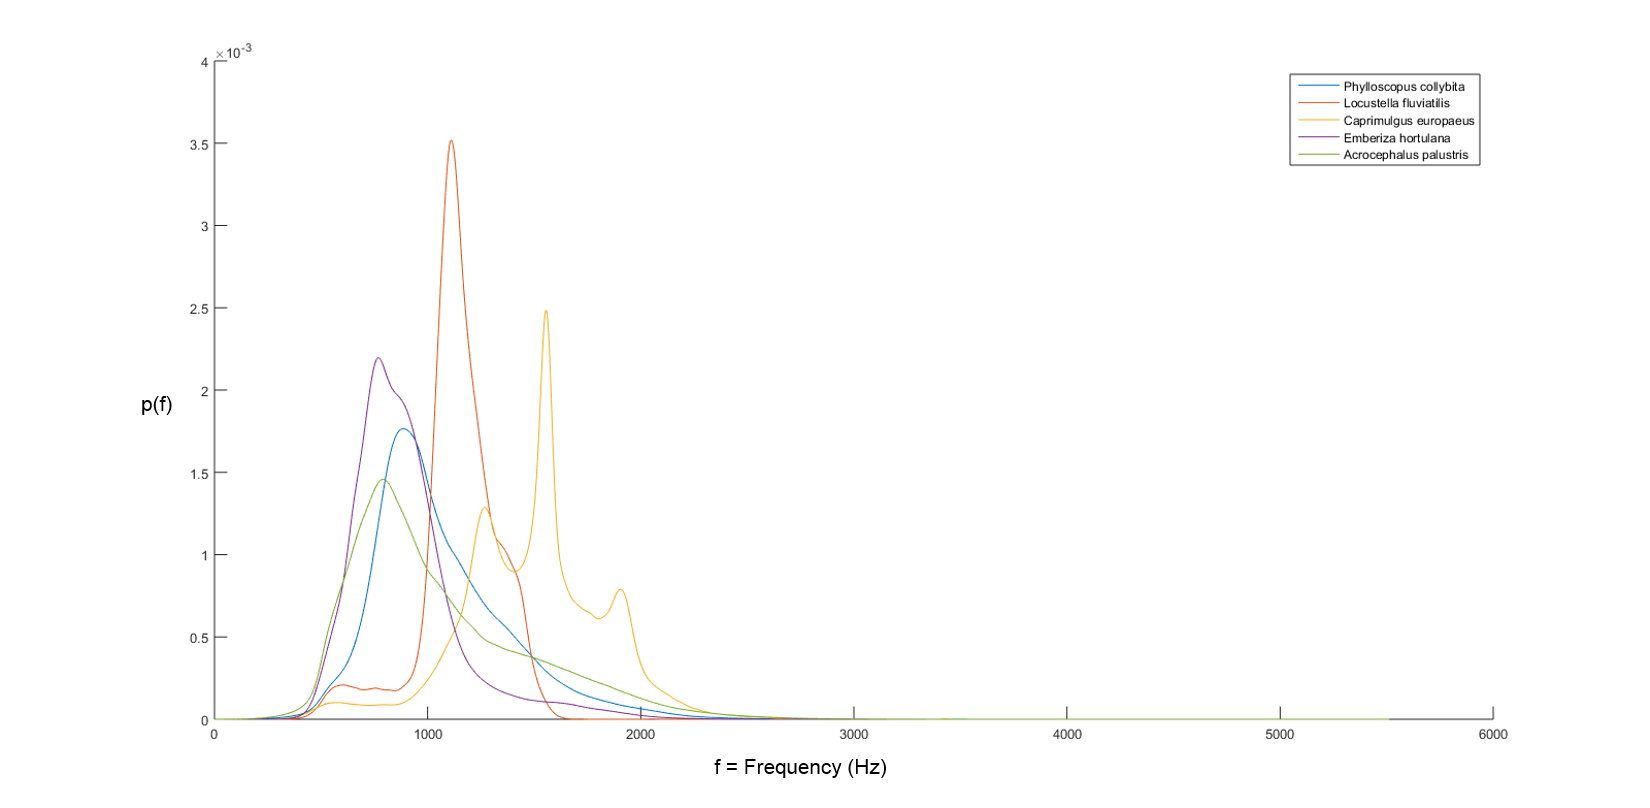
\includegraphics[width=\textwidth]{images/kdespecies}
\caption{Comparison of probability distributions generated by KDE for 5 different species. Despite having high probability in similar ranges of frequencies, their shapes are still distinguishable. }
\label{fig_kdespecies}
\end{figure}
\par Concerning VB-HMMs, we used the implementation of the Oxford Machine Learning Research Group, HMMBOX 4.1, which requires the NETLAB package. The former contains implementations of the tools required for a Bayesian treatment of HMMs, in particular: implementation of closed forms for the KL-divergence of the Normal, Dirichlet and Wishart distributions, variational inference training and sequence decoding. Furthermore, a routine that computes the occupancy of an HMM $\Omega_\lambda$ with respect to a sequence $\V{x}$ was also implemented. After computing the formant trajectories for each recording, the ones corresponding to a single species were concatenated and used as the training sequence for each HMM, i.e. we trained one HMM per species, and then computed their occupancy with respect to their respective training sequences. We used a Gaussian observation model for every HMM.
\par All the similarity metrics described in section \ref{section_model} were implemented as MATLAB scripts as well. Finally, the MATLAB Statistics and Machine Learning Toolbox contains functions to perform linkage and dendrogram plotting from a similarity matrix.

\subsection{Results}
\label{section_results}
In this subsection, we present phylo-acoustic trees obtained from using the techniques described in section \ref{section_model}. We first provide a qualitative assessment of these results, and then proceed to show formally that this data analysis does exhibit a clear structure. We used 6 different approaches to build phylo-acoustic trees:
\begin{itemize}
\item Symmetric KL Divergence over non-parametric distributions generated via KDE.
\item Hellinger distance over non-parametric distributions generated via KDE.
\item Symmetric KL Divergence over Gaussian Mixture Models trained as emission models for a Hidden Markov Model.
\item Hellinger distance over Gaussian Mixture Models trained as emission models for a Hidden Markov Model.
\item Symmetric KL Divergence over the Dirichlet distributions associated to the transition models of our Hidden Markov Models.
\item Occupancy-weighted Symmetric KL Divergence (as described in subsection \ref{sub_hmms}) over the Dirichlet distributions associated to the transition models of our Hidden Markov Models.
\end{itemize}
\par Full-size figures of each phylo-acoustic tree are offered below. Brown marks have been added to each figure whenever more than 40\% of a cluster consisted of species from the same genus (i.e. they share the first word in their scientific names). 
\begin{sidewaysfigure}[!ht]
\noindent\makebox[\textwidth]{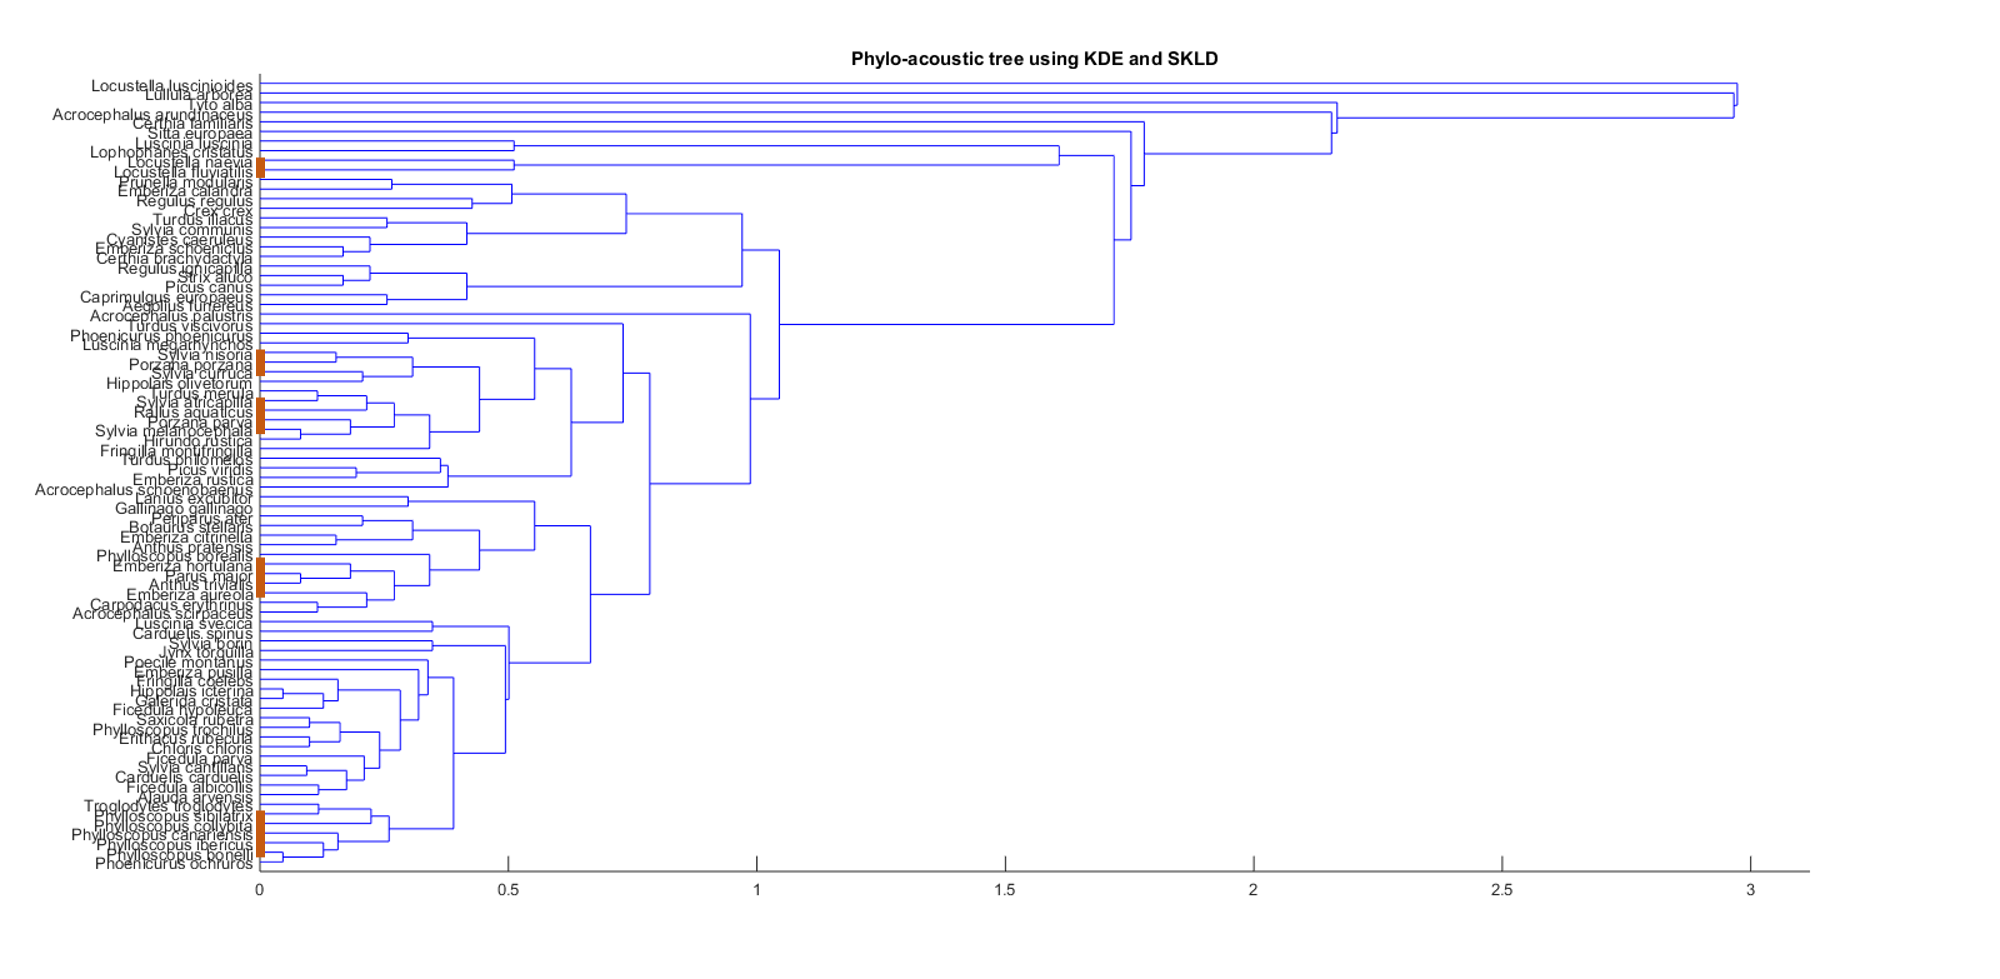
\includegraphics[width=\paperheight,height=18cm]{images/kde_skld_2}}
    \caption{Phylo-acoustic tree generated using the Symmetric KL Divergence between pairs of non-parametric distributions generated using KDE.}
    \label{fig:kdeskld}
\end{sidewaysfigure}


\begin{sidewaysfigure}[!ht]
\noindent\makebox[\textwidth]{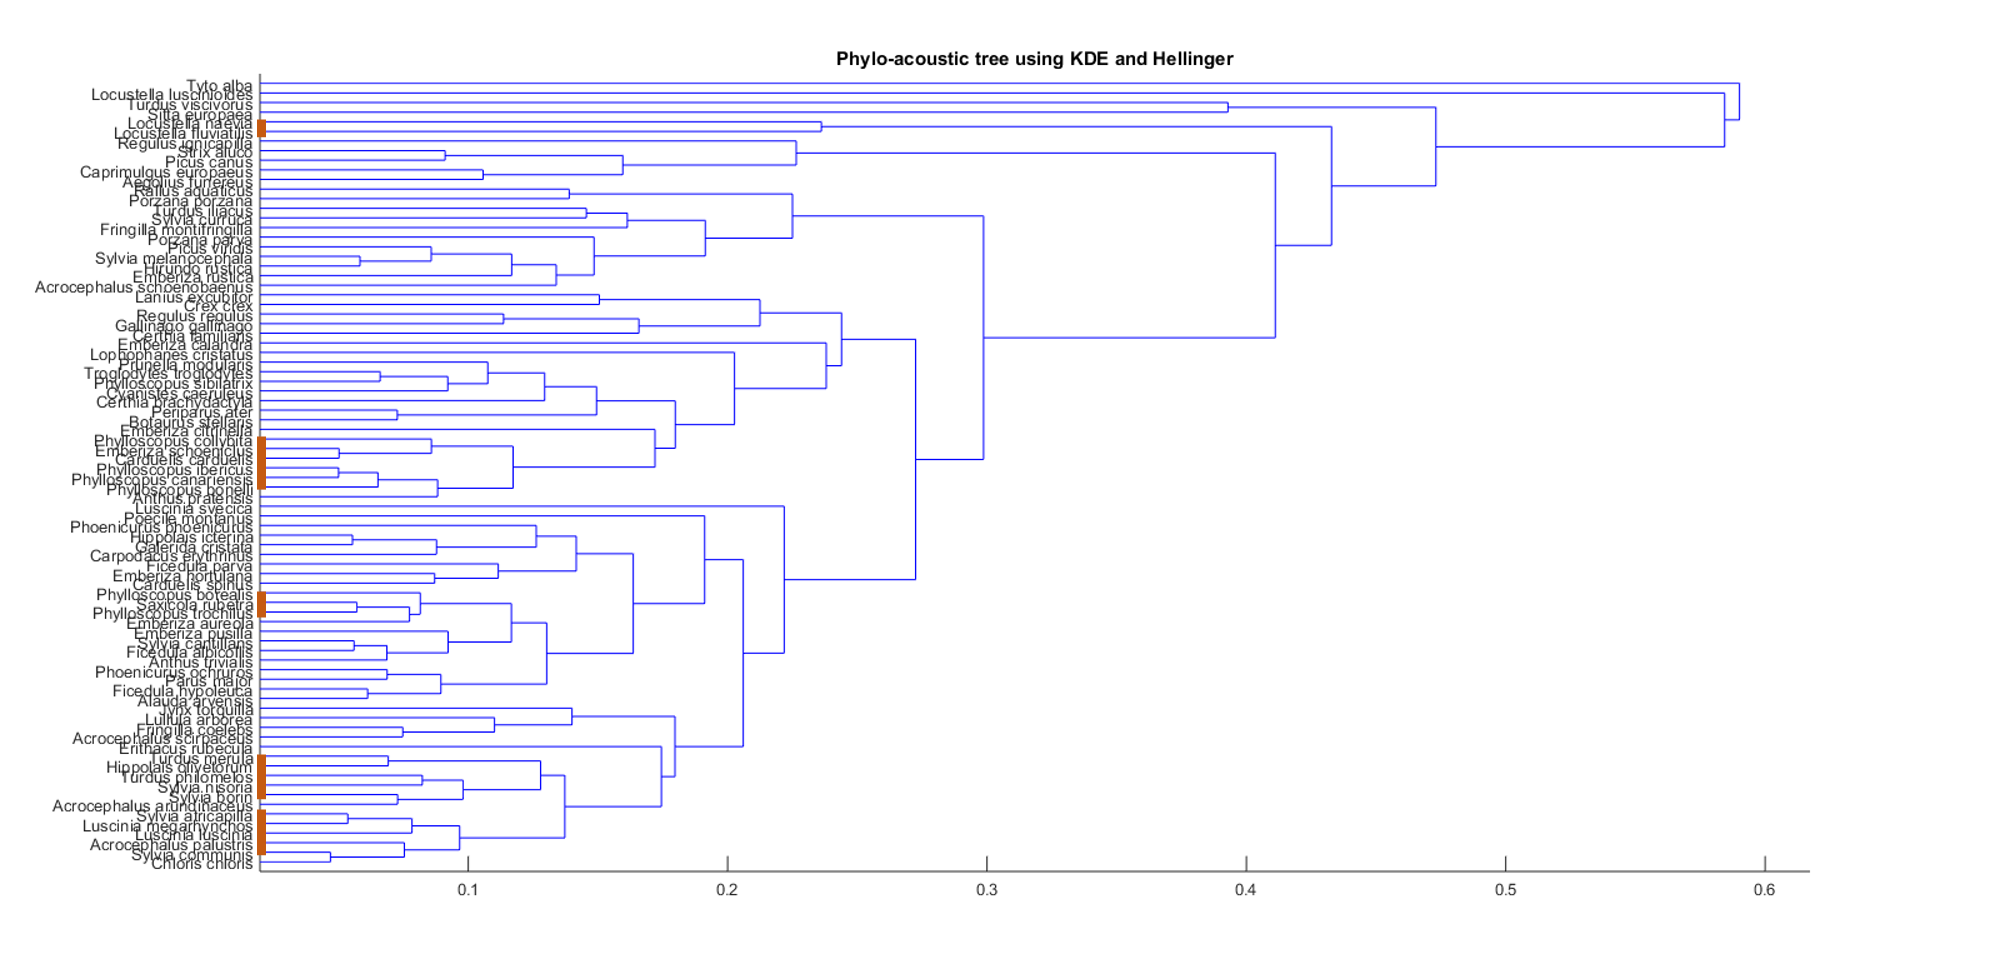
\includegraphics[width=\paperheight,height=18cm]{images/kde_hellinger_2}}
    \caption{Phylo-acoustic tree generated using the Hellinger distance between pairs of non-parametric distributions generated using KDE.}
    \label{fig:kdehellinger}
\end{sidewaysfigure}


\begin{sidewaysfigure}[!ht]
\noindent\makebox[\textwidth]{\includegraphics[width=\paperheight,height=18cm]{images/gmm_skld_2}}
    %\includegraphics[width=\textwidth]{gmm_skld_2}
    \caption{Phylo-acoustic tree generated using the Symmetric KL-Divergence between pairs of emission models (GMMs) from HMMs.}
    \label{fig:gmmskld}
\end{sidewaysfigure}


\begin{sidewaysfigure}[!ht]
\noindent\makebox[\textwidth]{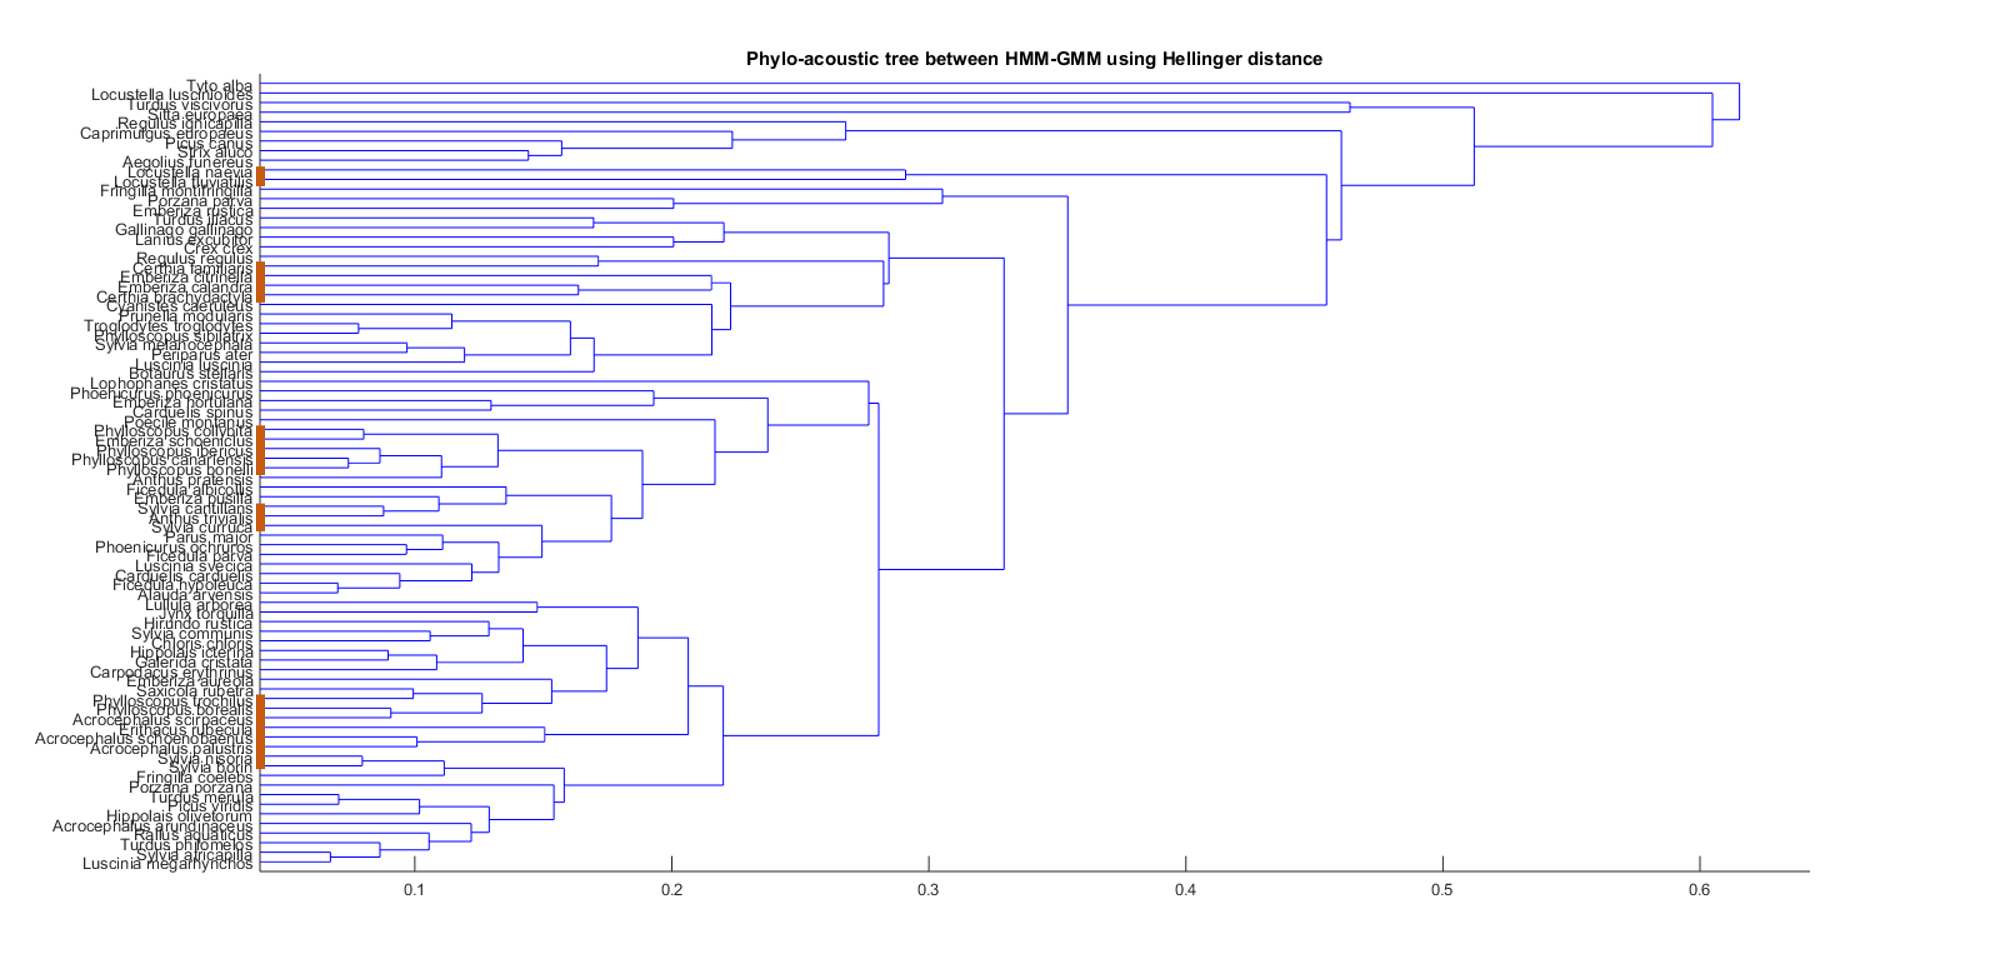
\includegraphics[width=\paperheight,height=18cm]{images/gmm_hellinger_2}}
    \caption{Phylo-acoustic tree generated using the Hellinger distance between pairs of emission models (GMMs) from HMMs.}
    \label{fig:gmmhellinger}
\end{sidewaysfigure}


\begin{sidewaysfigure}[!ht]
\noindent\makebox[\textwidth]{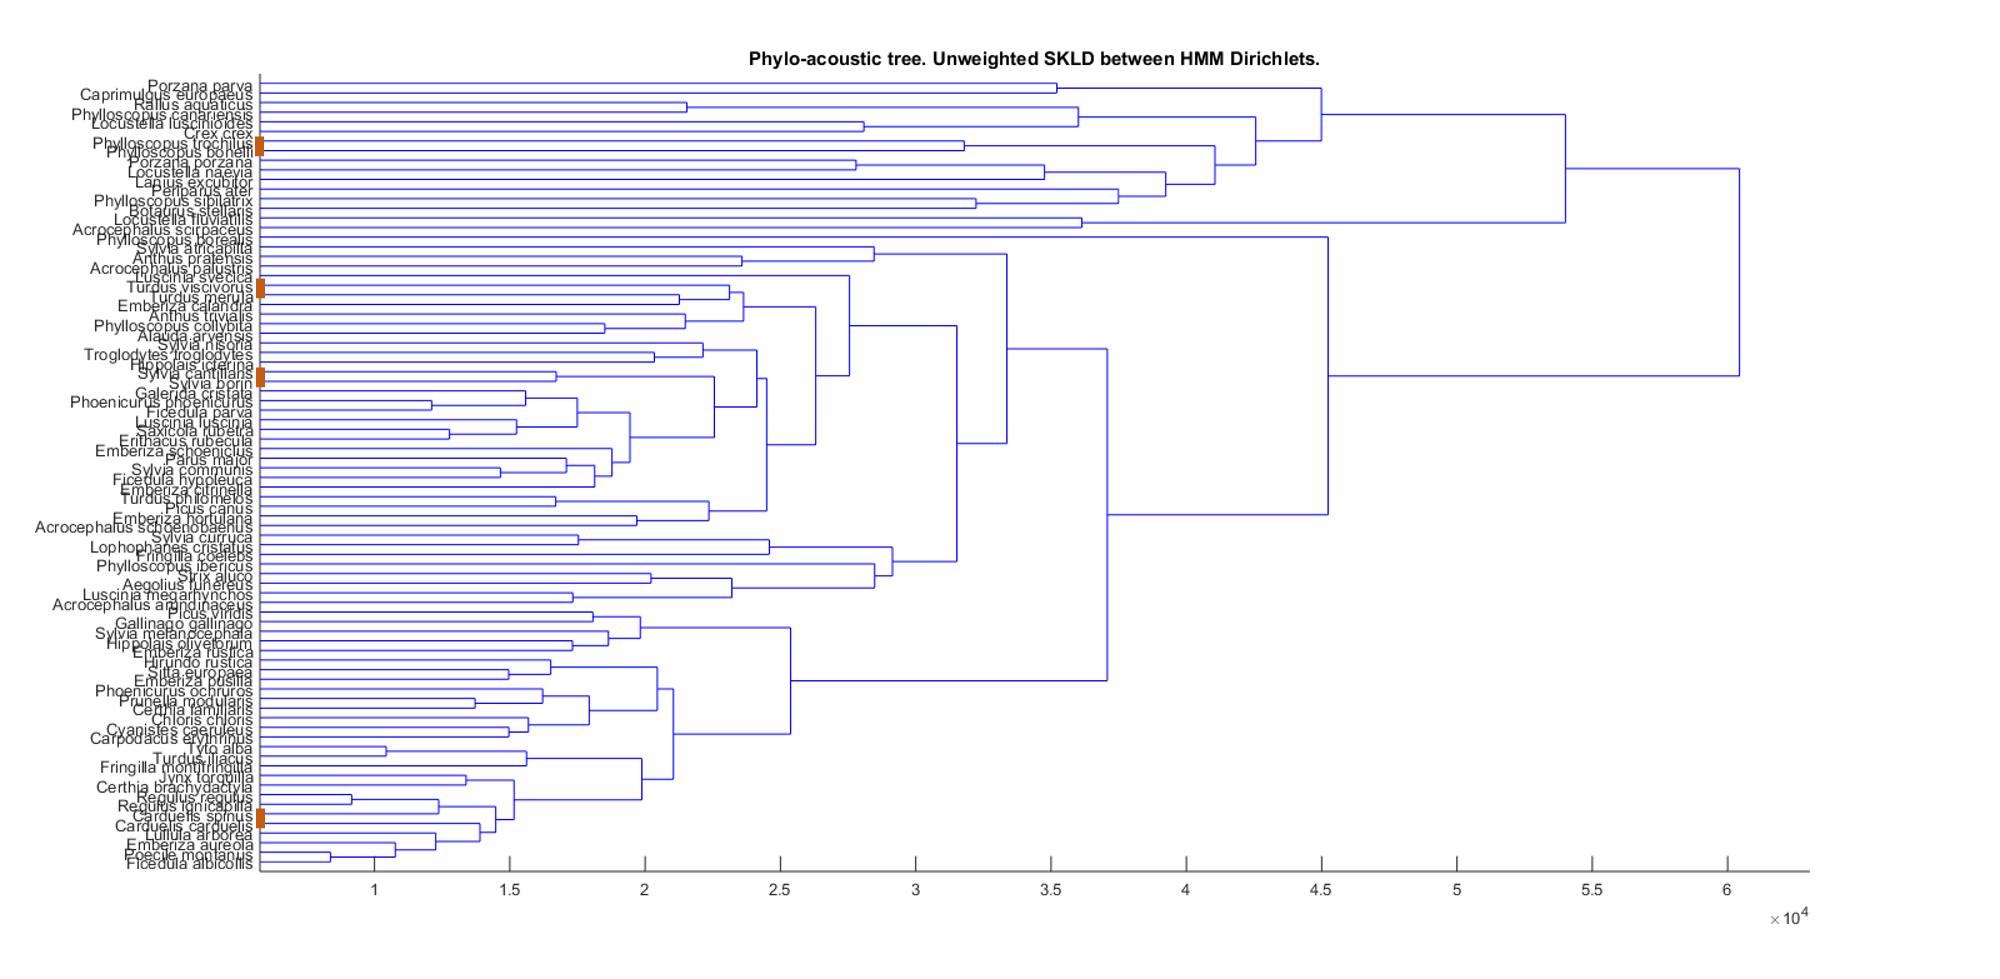
\includegraphics[width=\paperheight,height=18cm]{images/dirichlet_unweighted_2}}
    \caption{Phylo-acoustic tree generated using the Symmetric KL-Divergence between pairs of transition models (Dirichlets) from HMMs.}
    \label{fig:hmmunweighted}
\end{sidewaysfigure}


\begin{sidewaysfigure}[!ht]
\noindent\makebox[\textwidth]{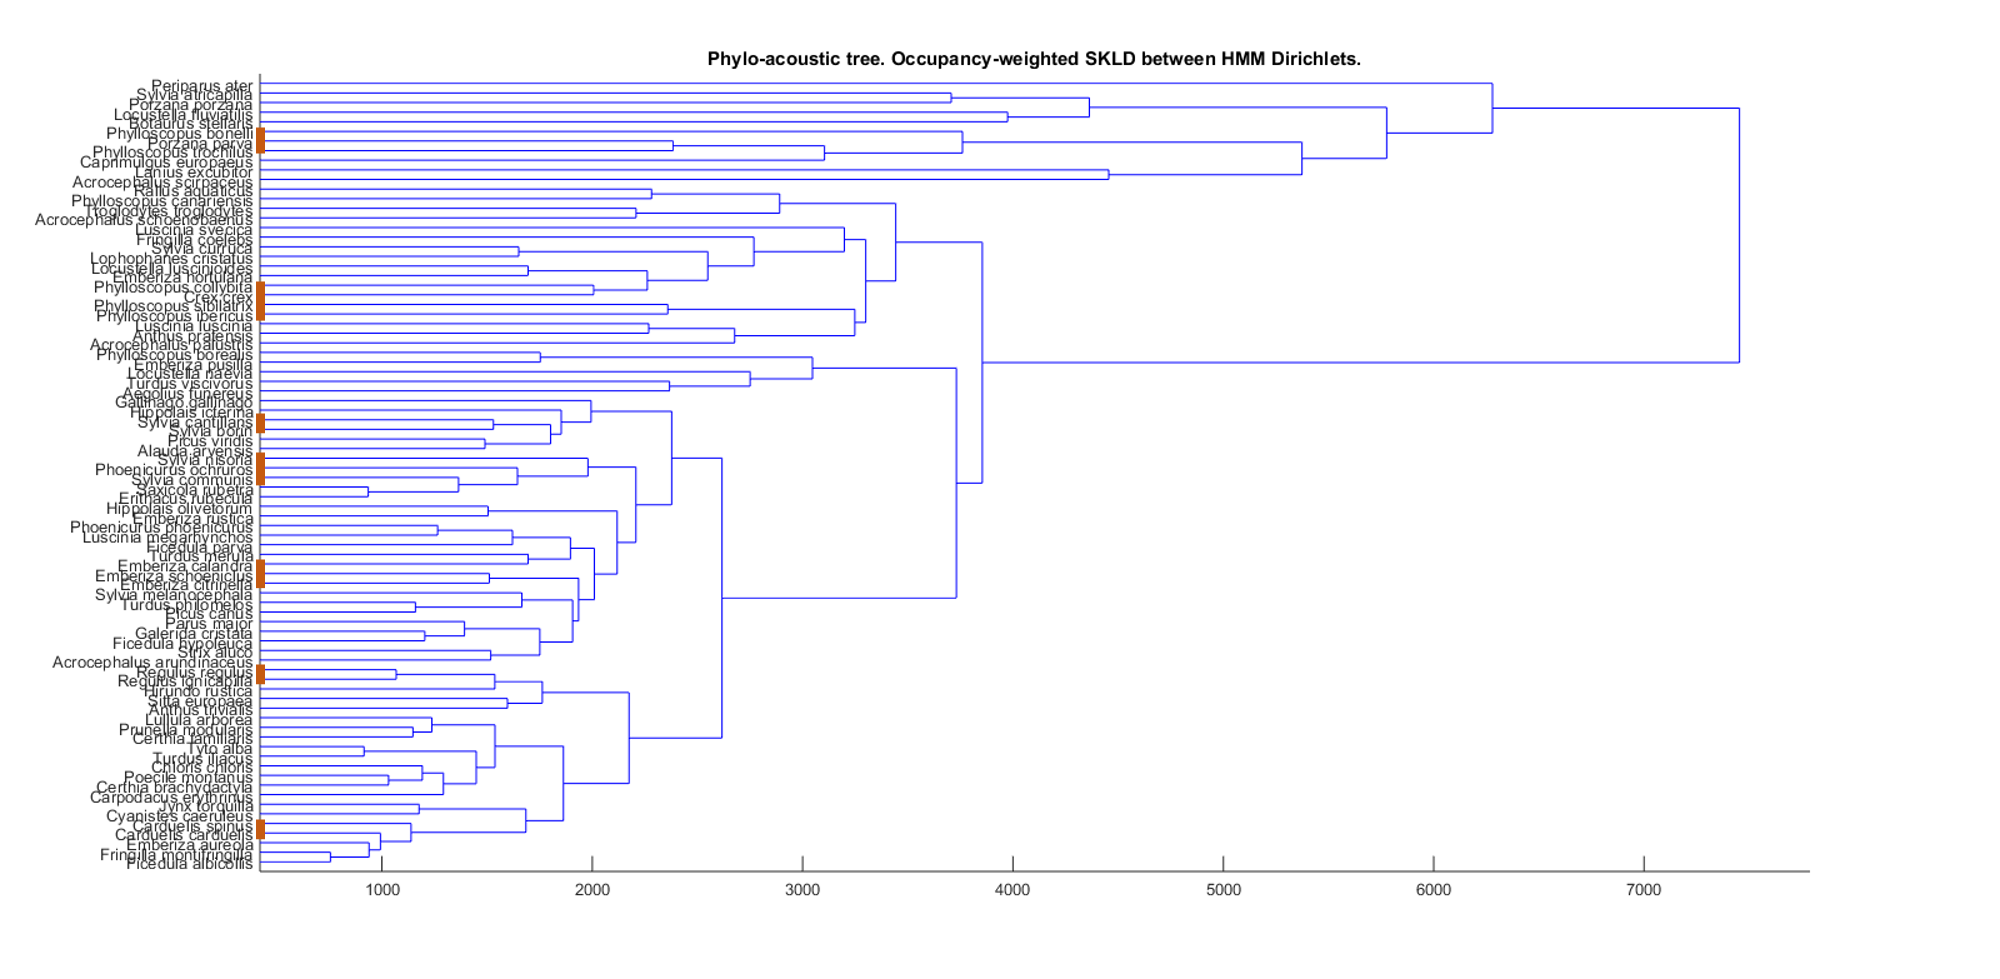
\includegraphics[width=\paperheight,height=18cm]{images/dirichlet_occupancy_2}}
    \caption{Phylo-acoustic tree generated using the occupancy-weighted Symmetric KL-Divergence between pairs of transition models (Dirichlets) from HMMs.}
    \label{fig:hmmweighted}
\end{sidewaysfigure}
\clearpage
\par These trees can be assessed in several ways - choosing to mark clusters whose species share an ancestor is just one of them. The versatility of this approach suggests that, rather than proving that facts from Zoology extend to Acoustic Analysis, we can change the focus and contribute to these facts by showing empirical evidence about relationships that could be unexpected from their point of view.
\par This key point was briefly discussed in section \ref{section_introduction}, when we argued that birds sharing common ancestors need not necessarily share birdsong traits in the future. Birdsong is not uniquely determined by genes, instead it often suffers modifications that are due to mating advantage and adaptation to new environments. For this reason, relations unveiled in phylo-acoustic trees could also be linked to migration patterns and, more generally, geolocalisation.
\par Nevertheless, one of the most important conclusions we aim to draw from these trees is that their structure is no coincidence. To achieve this, we aim to disprove the null hypothesis:
\begin{align*}
H_0 = \text{there is no relationship between the species in a phylo-acoustic tree.}
\end{align*}
\par If this hypothesis is true, then randomly generated data has the same structure as any of these trees. To generate such data, we sample random formant trajectories from the uniform distribution $\mathcal{U}(f_{min}, f_{max})$, where the boundaries of the distribution correspond to the minimum and maximum formant seen in any species in the dataset. After generating as many formant trajectories as bird species, we generate new ``phylo-acoustic trees'' for each of them. The resulting trees are shown below.
\begin{sidewaysfigure}[!ht]
\noindent\makebox[\textwidth]{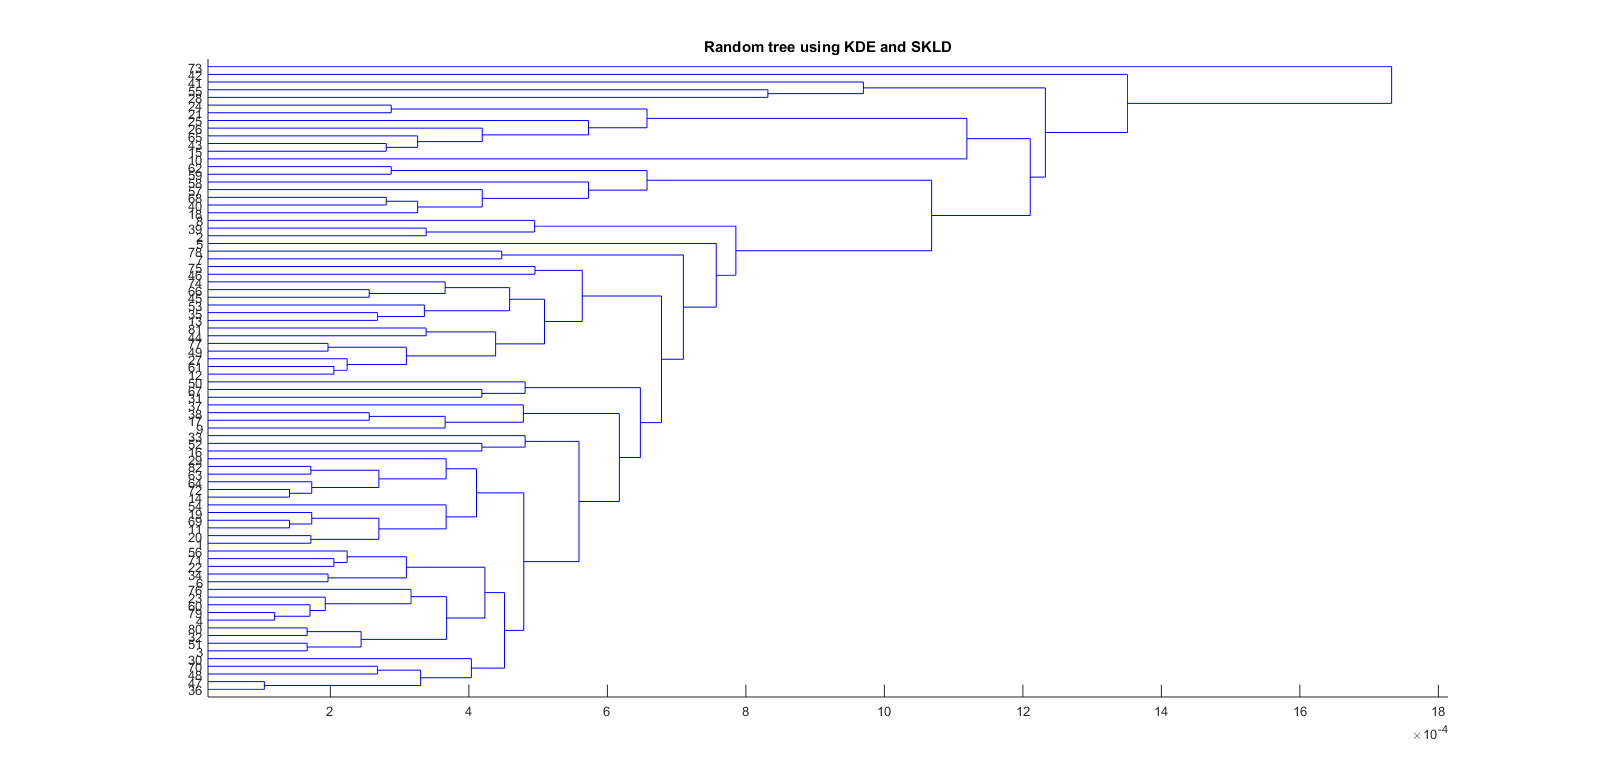
\includegraphics[width=\paperheight,height=18cm]{images/random_kde_skld}}
    \caption{Random phylo-acoustic tree generated using the Symmetric KL Divergence between pairs of non-parametric distributions generated using KDE.}
    \label{fig:rkdeskld}
\end{sidewaysfigure}


\begin{sidewaysfigure}[!ht]
\noindent\makebox[\textwidth]{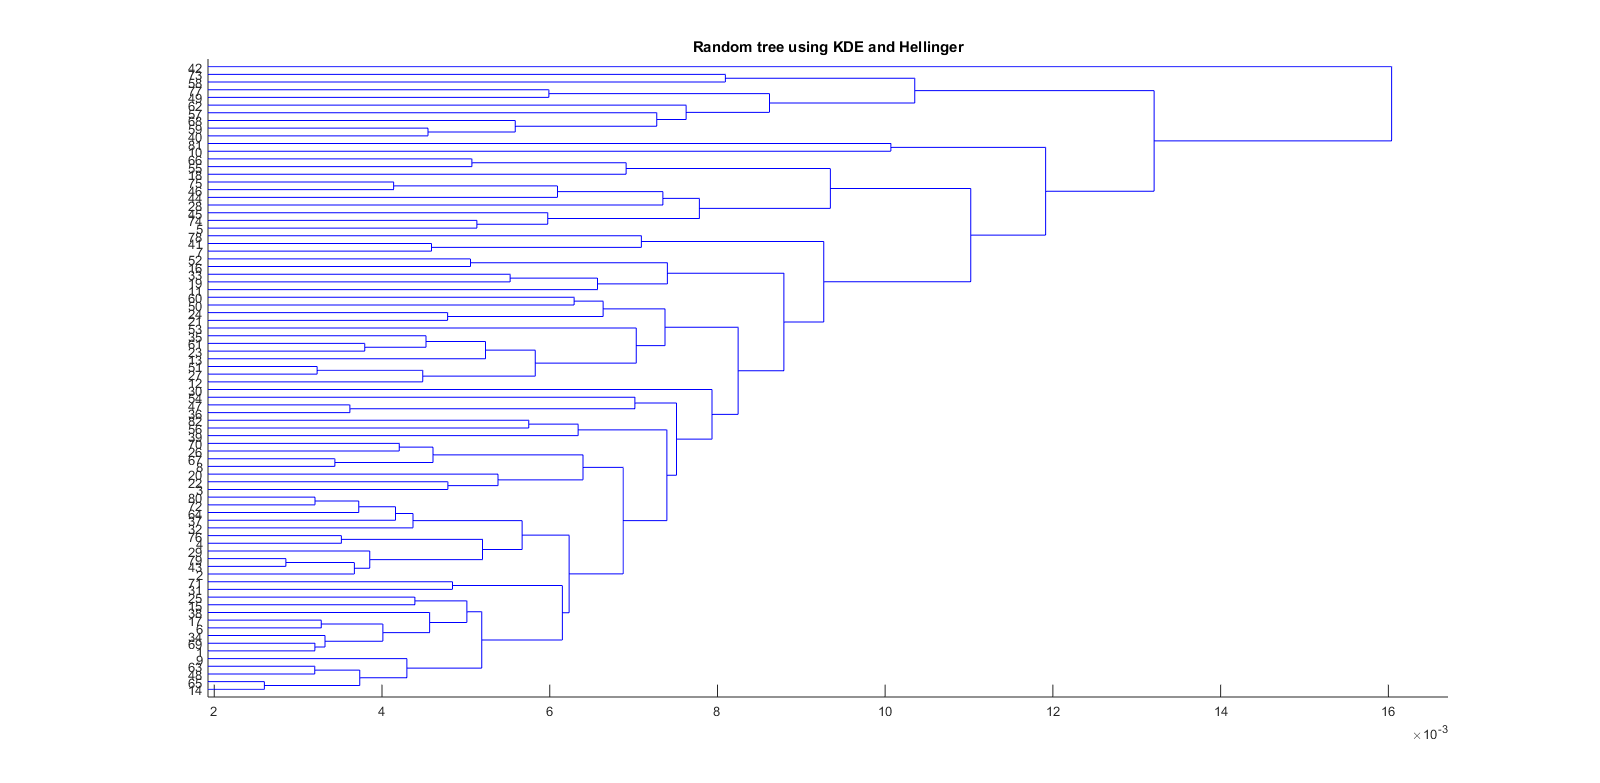
\includegraphics[width=\paperheight,height=18cm]{images/random_kde_hellinger}}
    \caption{Random phylo-acoustic tree generated using the Hellinger distance between pairs of non-parametric distributions generated using KDE.}
    \label{fig:rkdehellinger}
\end{sidewaysfigure}


\begin{sidewaysfigure}[!ht]
\noindent\makebox[\textwidth]{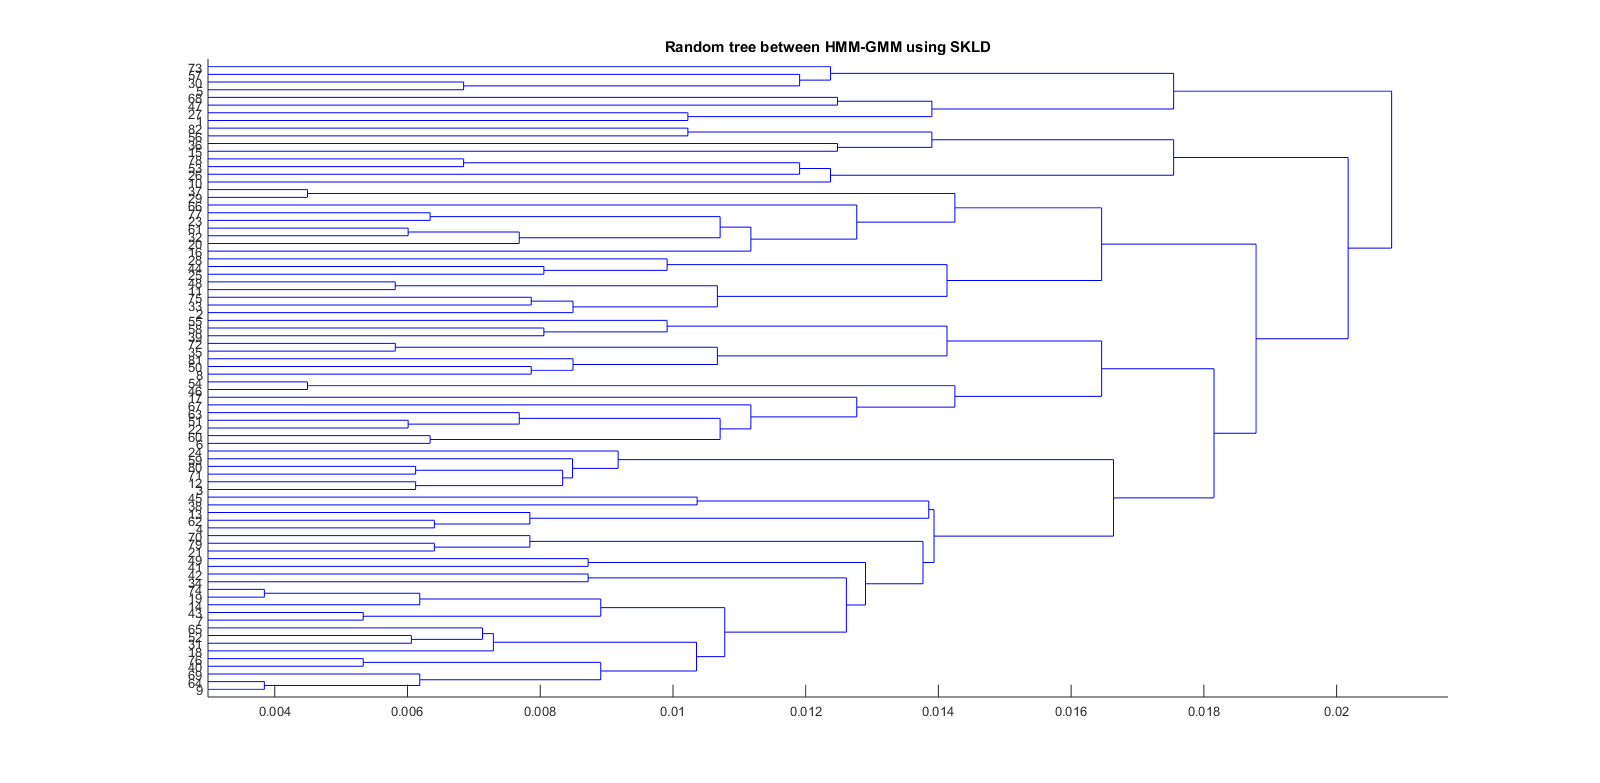
\includegraphics[width=\paperheight,height=18cm]{images/random_gmm_skld}}
    \caption{Random phylo-acoustic tree generated using the Symmetric KL-Divergence between pairs of emission models (GMMs) from HMMs.}
    \label{fig:rgmmskld}
\end{sidewaysfigure}


\begin{sidewaysfigure}[!ht]
\noindent\makebox[\textwidth]{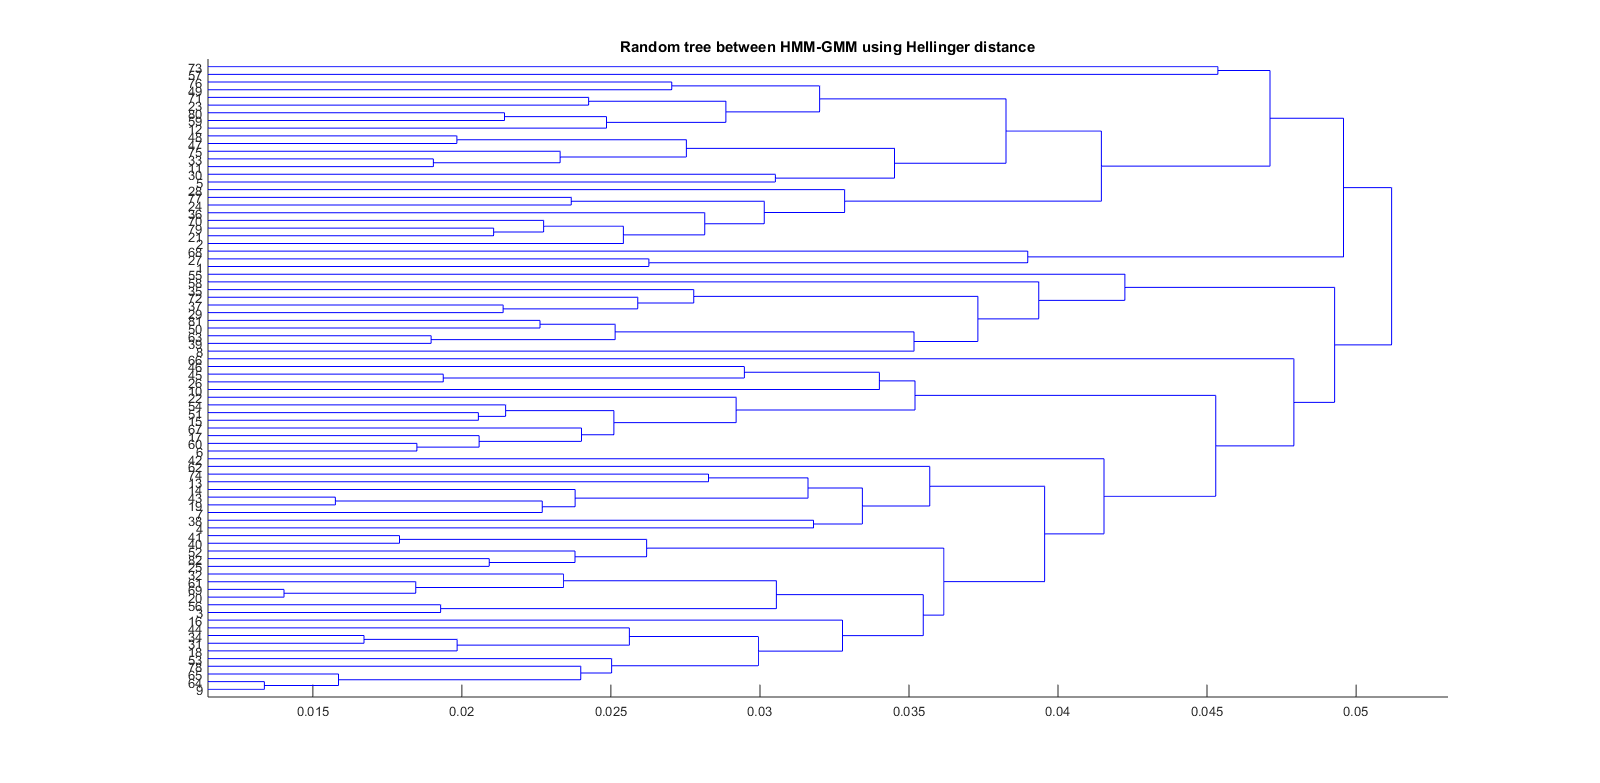
\includegraphics[width=\paperheight,height=18cm]{images/random_gmm_hellinger}}
    \caption{Random phylo-acoustic tree generated using the Hellinger distance between pairs of emission models (GMMs) from HMMs.}
    \label{fig:rgmmhellinger}
\end{sidewaysfigure}


\begin{sidewaysfigure}[!ht]
\noindent\makebox[\textwidth]{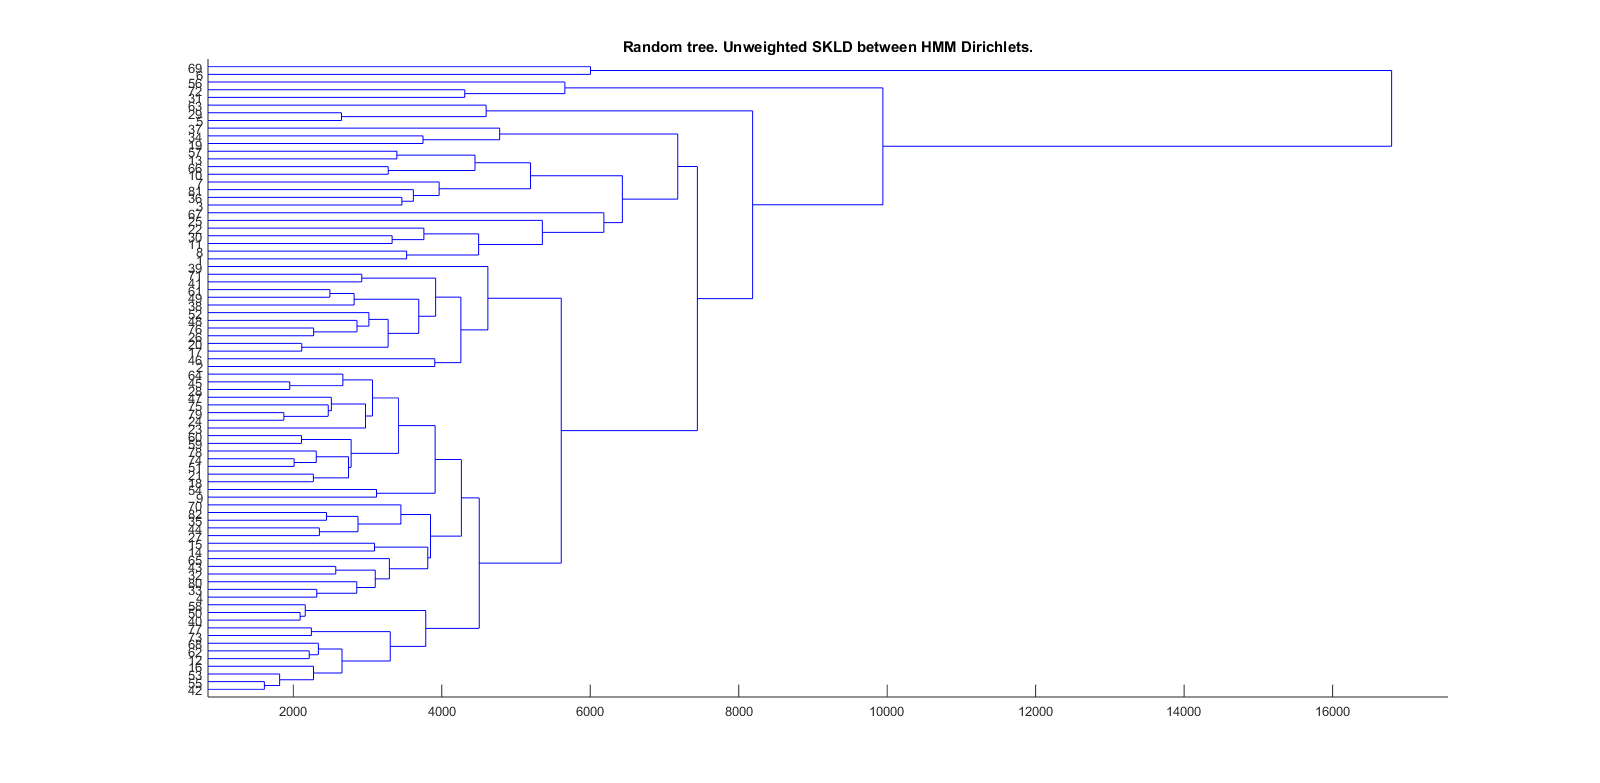
\includegraphics[width=\paperheight,height=18cm]{images/random_dirichlet_unweighted}}
    \caption{Random phylo-acoustic tree generated using the Symmetric KL-Divergence between pairs of transition models (Dirichlets) from HMMs.}
    \label{fig:rhmmunweighted}
\end{sidewaysfigure}

\begin{sidewaysfigure}[!ht]
\noindent\makebox[\textwidth]{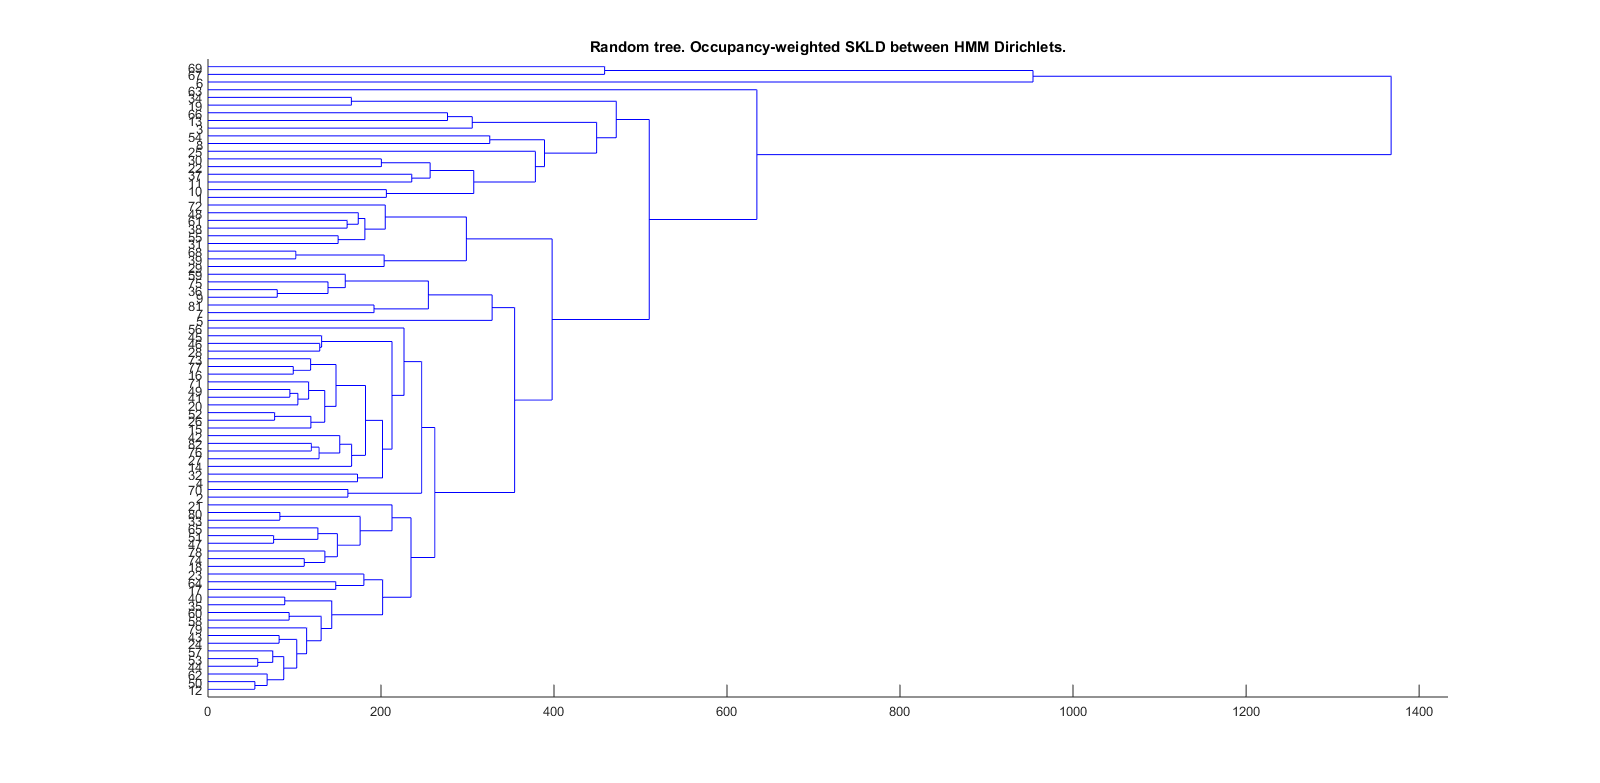
\includegraphics[width=\paperheight,height=18cm]{images/random_dirichlet_occupancy}}
    \caption{Random phylo-acoustic tree generated using the occupancy-weighted Symmetric KL-Divergence between pairs of transition models (Dirichlets) from HMMs.}
    \label{fig:rhmmweighted}
\end{sidewaysfigure}
\clearpage

\par We compare each pair of trees generated using the same technique by plotting how the number of clusters changes through time. When there is real structure in data, clusters are tight and well separated from each other. This implies the distance between clusters becomes larger as smaller clusters merge. This maps visually to long branches in a dendrogram. On the other hand, when there is no real structure in data, objects tend to be similar distances apart from each other (they are uniformly scattered in space). When a new cluster is formed, linkage methods tend to change very little the distances between the original clusters, since they were very similar before merging. This translates into clusters that have a short life.
\par The dendrogram is not a representation suitable to compare structured and non-structured data in parallel. Instead, we plot the lifetime (from 0 up to the lifetime of the longest-living cluster) versus the number of clusters in each tree. In each plot, note the rate of change of the red curves (representing random structures) compared with the blue ones (real data). The red curves go down to zero very quickly, suggesting that clusters are merged at a fast rate; on the other hand, the blue lines do not only span a longer lifetime, but they also contain short horizontal segments that grow longer as time flows. This suggests that it takes longer for clusters to merge as the number of remaining clusters decreases. This is consistent with our hypothesis: at the beginning, many clusters belong to the same community, and thus they are clustered fairly quickly. However, as communities are formed, they lie further apart from each other, hence it takes longer for them to fuse.
\par We obtain similar results in all six cases. The red curves depicting the random statistical models go down very quickly due to clusters that live too little, as opposed to the blue lines (real data), which live many orders of magnitude longer. These findings are strong arguments to reject the null hypothesis and hence conclude that real data does exhibit real structure.
\begin{figure}[H]
\centering
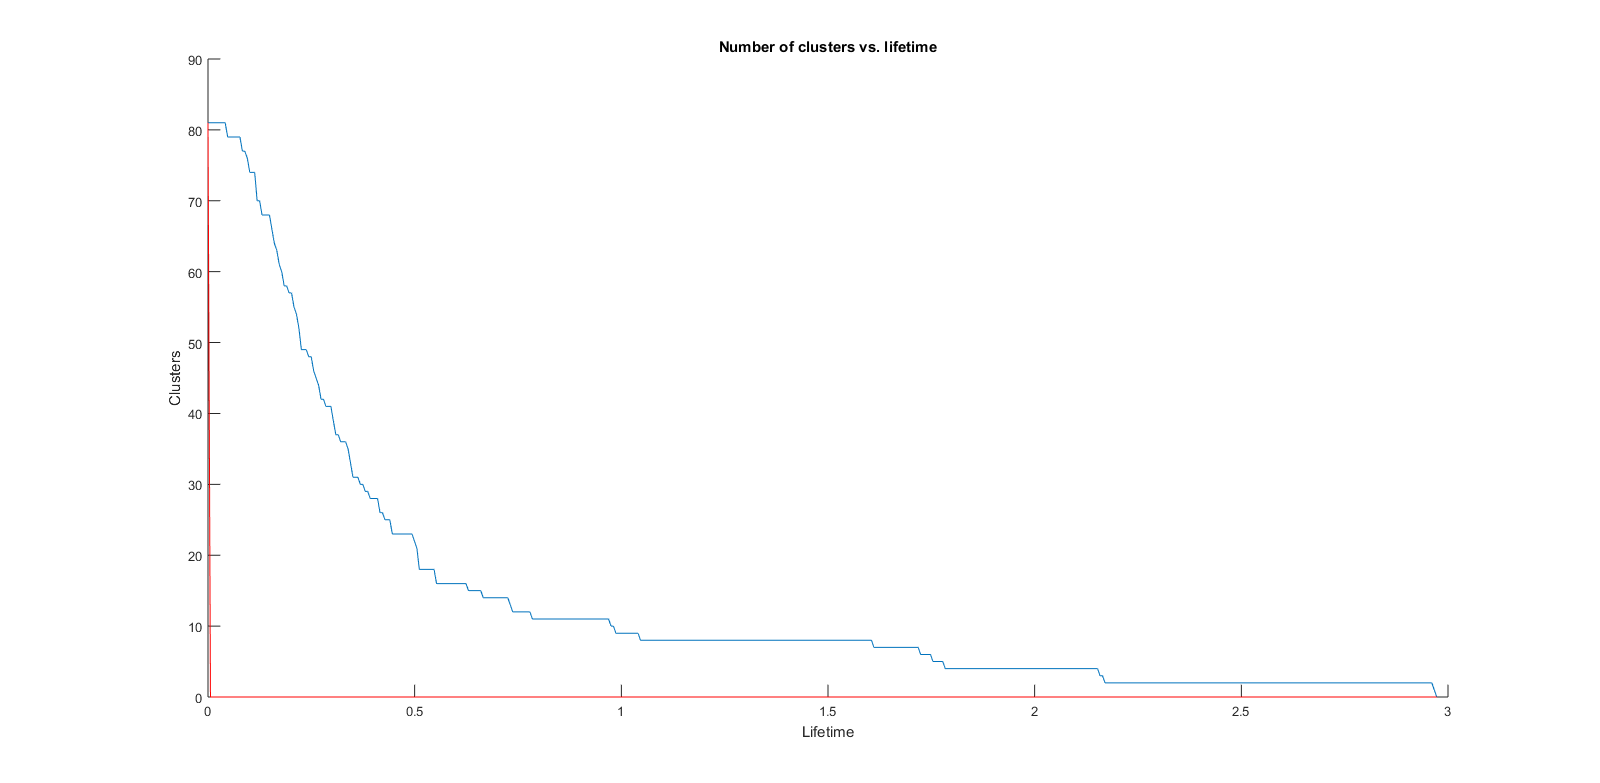
\includegraphics[width=\textwidth]{images/lifetime_kde_skld}
\caption{Lifetime vs. number of clusters using the Symmetric KL Divergence between non-parametric distributions obtained via KDE.}
\label{fig_lt_kde_skld}
\end{figure}

\begin{figure}[H]
\centering
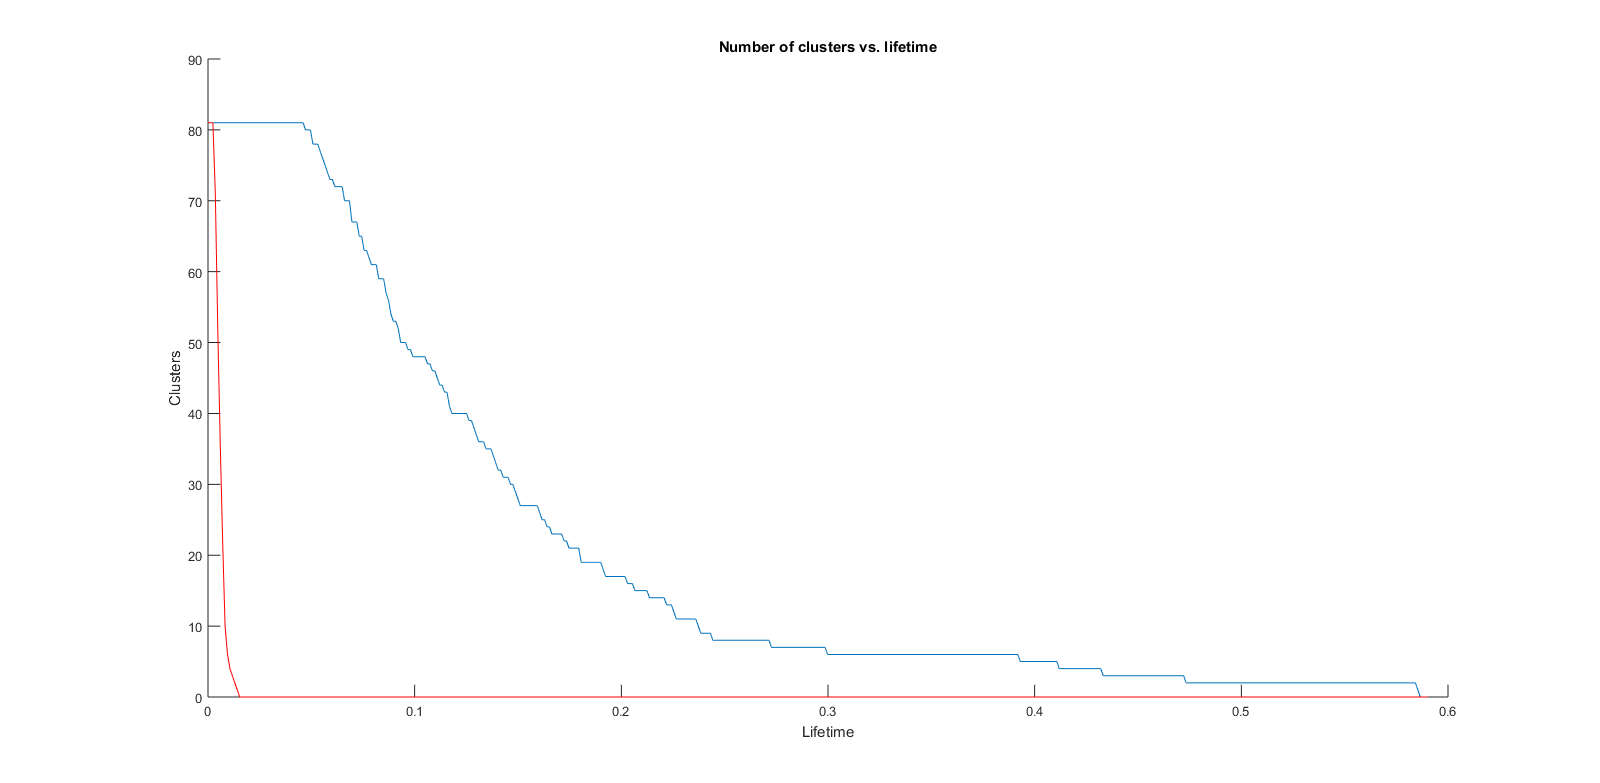
\includegraphics[width=\textwidth]{images/lifetime_kde_hellinger}
\caption{Lifetime vs. number of clusters using the Hellinger distance between non-parametric distributions obtained via KDE.}
\label{fig_lt_kde_hellinger}
\end{figure}

\begin{figure}[H]
\centering
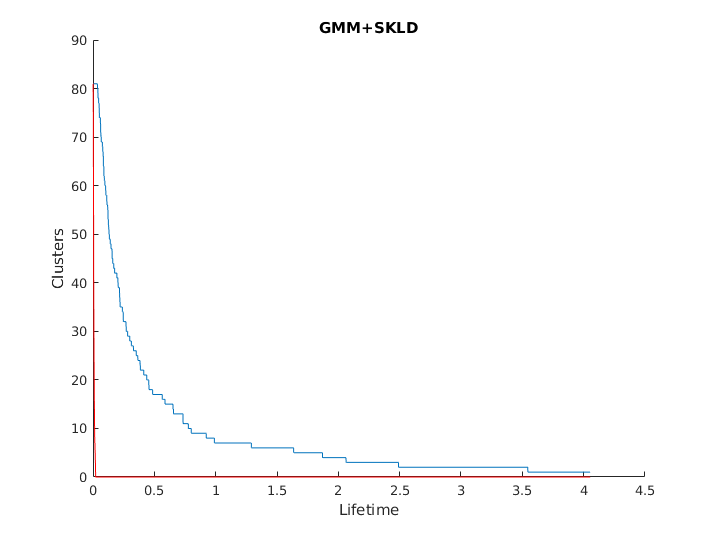
\includegraphics[width=\textwidth]{images/lifetime_gmm_skld}
\caption{Lifetime vs. number of clusters using the Symmetric KL Divergence between HMM emission models (GMMs).}
\label{fig_lt_gmm_skld}
\end{figure}

\begin{figure}[H]
\centering
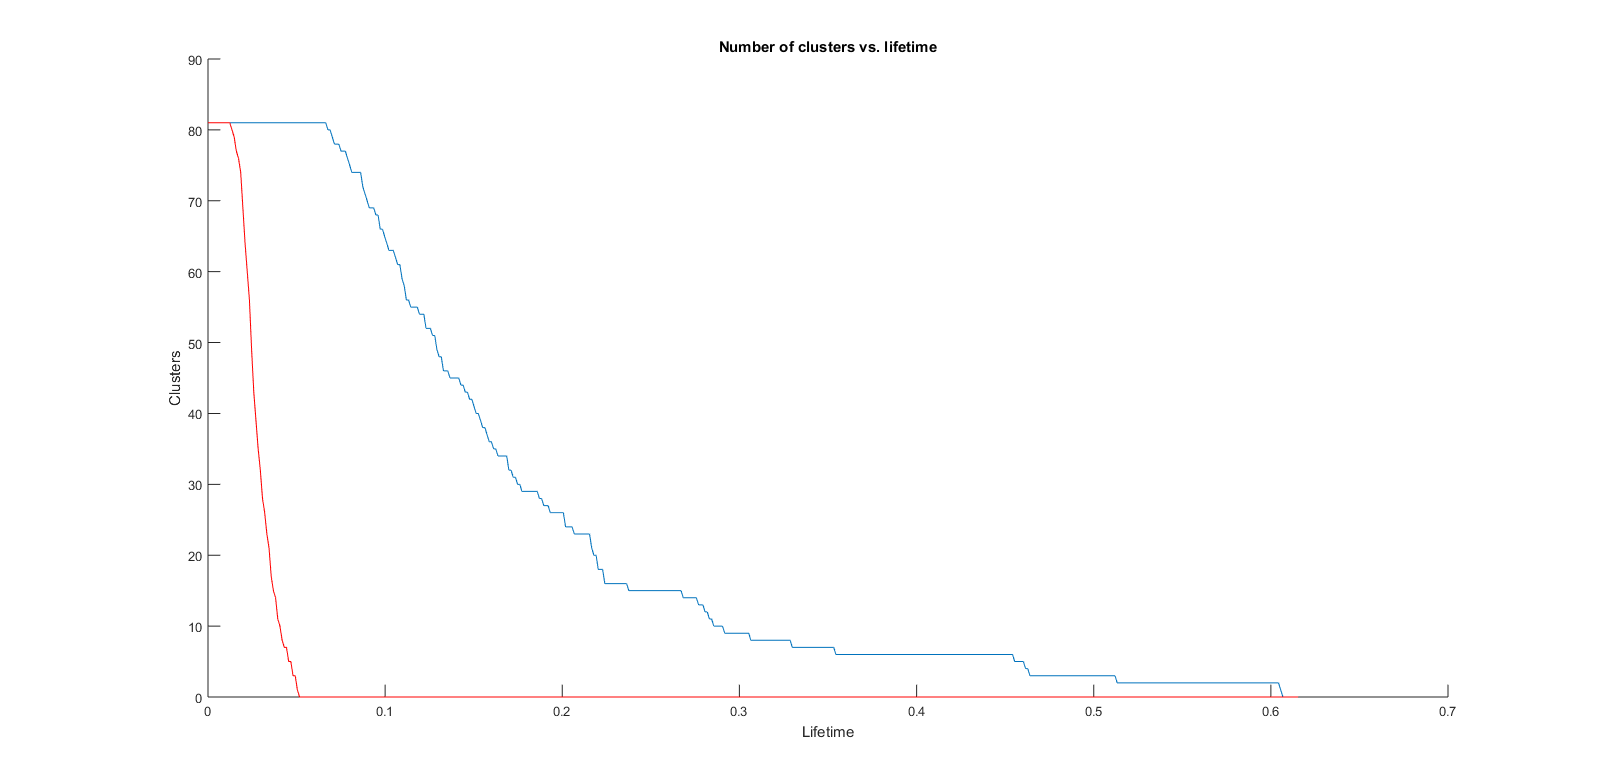
\includegraphics[width=\textwidth]{images/lifetime_gmm_hellinger}
\caption{Lifetime vs. number of clusters using the Hellinger distance between HMM emission models (GMMs).}
\label{fig_lt_gmm_hellinger}
\end{figure}

\begin{figure}[H]
\centering
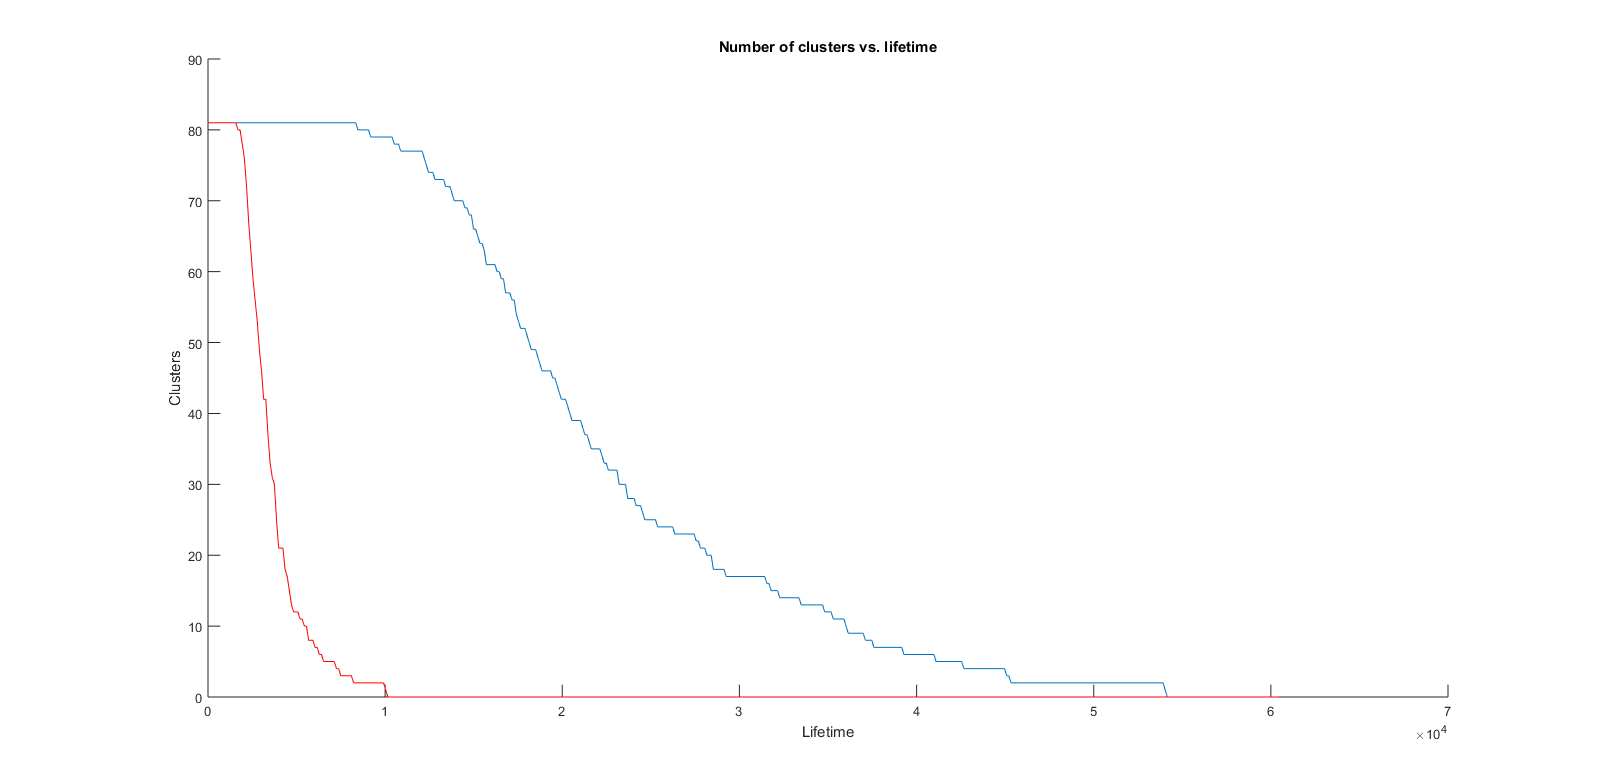
\includegraphics[width=\textwidth]{images/lifetime_dirichlet_unweighted}
\caption{Lifetime vs. number of clusters using the Dirichlet distance between HMMs.}
\label{fig_lt_du}
\end{figure}

\begin{figure}[H]
\centering
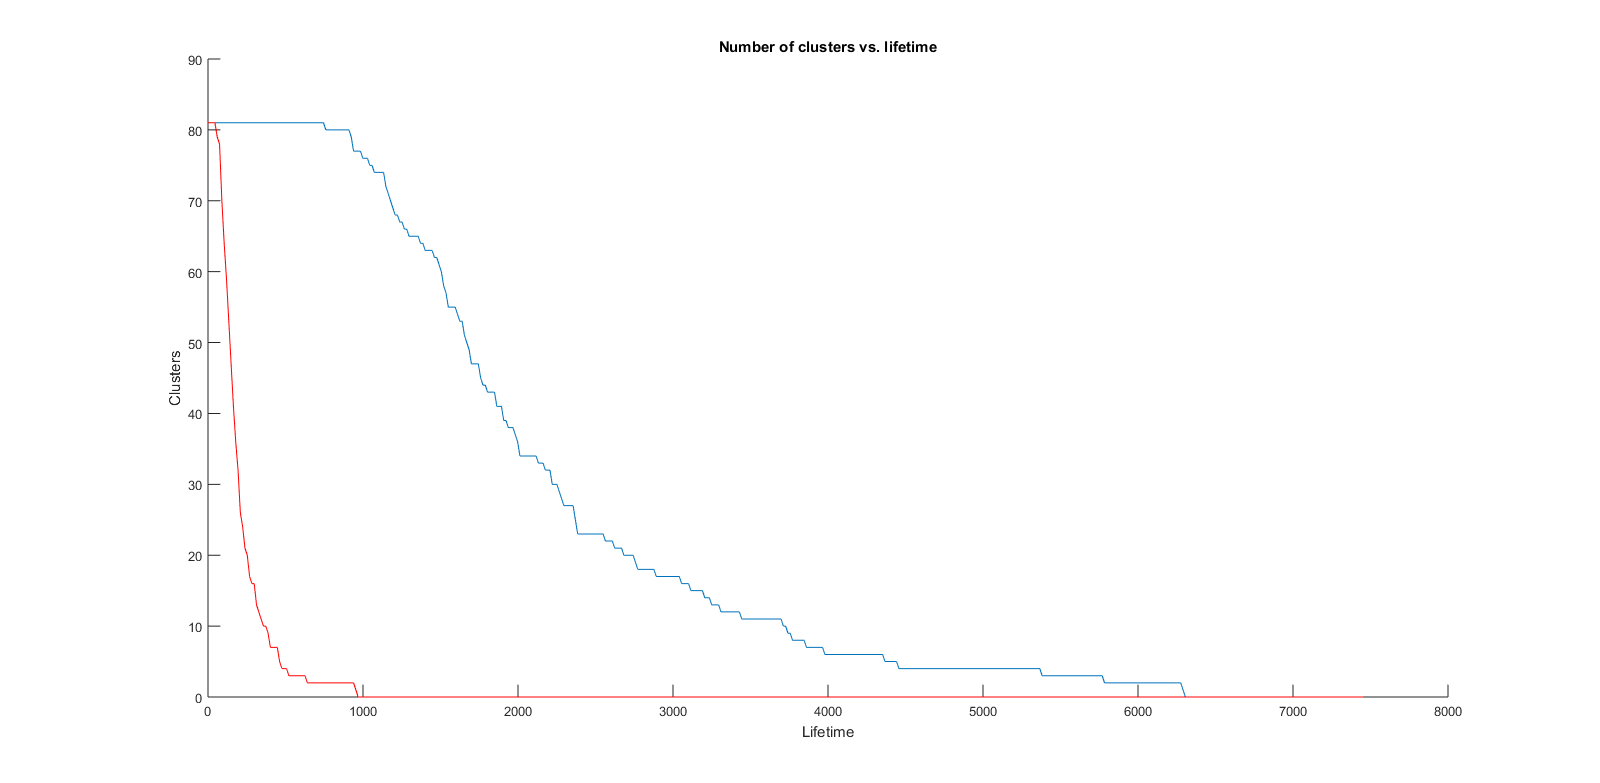
\includegraphics[width=\textwidth]{images/lifetimedirichlet_occupancy}
\caption{Lifetime vs. number of clusters using the Occupancy-weighted Dirichlet distance between HMMs.}
\label{fig_lt_occ}
\end{figure}   


\section{Conclusion (500 words)}
\label{section_conclusion}



\section*{Acknowledgements}


The authors would like to thank the National Council for Science and Technology in Mexico (CONACYT) for funding this research project.


\addcontentsline{toc}{chapter}{Bibliography}
\bibliographystyle{unsrt}
\bibliography{bib}

\end{document}


